%!TEX TS-program = xelatex 
%!TEX TS-options = -synctex=1 -output-driver="xdvipdfmx -q -E"
%!TEX encoding = UTF-8 Unicode
%
%  formwithoutmatter
%
%  Created by Mark Eli Kalderon on 2011-03-05.
%  Copyright (c) year. All rights reserved.
%

\documentclass[12pt]{book} 

% Definitions
\newcommand\mykeywords{Aristotle, perception, color}
\newcommand\myauthor{Mark Eli Kalderon}

% Packages
\usepackage{geometry} \geometry{a4paper} 
\usepackage{url}
\usepackage{txfonts}
\usepackage{color}
\usepackage{enumerate}
\usepackage{tikz}
\definecolor{gray}{rgb}{0.459,0.438,0.471}

% XeTeX
\usepackage[cm-default]{fontspec}
\usepackage{xltxtra,xunicode}
\defaultfontfeatures{Scale=MatchLowercase,Mapping=tex-text}
\setmainfont{Hoefler Text}

% Bibliography
\usepackage[round]{natbib} 

% Title Information
\title{Form without Matter\\
Aristotle on Color Perception}
\author{\myauthor} 
% \date{} % Leave blank for no date, comment out for most recent date

% PDF Stuff
\usepackage[plainpages=false, pdfpagelabels, bookmarksnumbered, backref, pdftitle={Form Without Matter}, pagebackref, pdfauthor={\myauthor}, pdfkeywords={\mykeywords}, xetex, dvipdfmx, colorlinks=true, citecolor=gray, linkcolor=gray, urlcolor=gray]{hyperref} 



%%% BEGIN DOCUMENT
\begin{document}

% Title Page
\maketitle
\vskip 2em \hrule height 0.4pt \vskip 2em


% Layout Settings
\setlength{\parindent}{1em}

% Main Content

\pagebreak
\tableofcontents

%!TEX root = /Users/markelikalderon/Documents/Git/formwithoutmatter/aristotle.tex
\chapter{Empedocles} % (fold)
\label{cha:empedocles}

\section{Dialectic} % (fold)
\label{sec:dialectic}

The present essay concerns Aristotle's dialectical engagement with Empedocles\index{Empedocles} about the nature of color perception. It is only by paying careful attention to such engagement can we arrive at a proper understanding of Aristotle's notorious definition of perception\index{perception!definition} as the assimilation\index{assimilation|seealso{perception!definition}} of the sensible form\index{form} without the matter\index{matter} of the perceived object. I shall argue that Aristotle's definition of perception is a resolution of a puzzle or \emph{aporia}\index{aporia@\emph{aporia}} about the nature of perception that animated Empedocles' theory of vision\index{Empedocles!perception}. The puzzle concerns the sensory presentation of remote sensible objects as when we see the brilliant white of the distant sun. This chapter details the original form of Empedoclean puzzlement\index{presentation!Empedoclean puzzlement} and shows how Empedocles' theory of vision is an attempt to resolve such puzzlement, though an attempt that, as we shall see in chapter~\ref{cha:perception_at_a_distance}, Aristotle rejects as unworkable. But before we discuss the puzzle which animates Empedocles' theory of color vision, it will be useful to briefly describe Aristotle's dialectical engagement with the \emph{endoxa} more generally.

Dialectical argument\index{dialectical argument} is a mode of reasoning that uses the \emph{endoxa}\index{endoxa@\emph{endoxa}} as premises. The \emph{endoxa} are the reputable opinions of one's predecessors. The reputable opinions:
\begin{quote}
	\ldots\ are accepted by everyone or by the majority or by the wise---i.e. by all, or by the majority, or by the most notable and reputable of them. (Aristotle, \emph{Topica} \textsc{i} 1 101\( ^{a} \)35--37; Pickard-Cambridge in \citealt[2-3]{Barnes:1984uq})\index{Topica@\emph{Topica}}
\end{quote}
The opinions of the many and the wise are the source of both truth and error. Dialectical argument contrasts, in this way, with geometrical demonstration\index{dialectical argument!contrasted with geometrical demonstration}. Geometrical demonstration begins, not with the opinions of predecessors which may be a source of truth or error, but with premises that are primitive truths.

That the relevant opinions are widespread or are offered by the wise at least makes it likely that some element of truth is to be found among them. This is important insofar as dialectical argument is an alethic activity\index{dialectical argument!as an alethic activity}:
\begin{quote}
	For the study of the philosophical sciences it is useful, because the ability to puzzle on both sides of a subject will make us detect more easily the truth and error about the several points that arise. (Aristotle, \emph{Topica} \textsc{i} 2 101\( ^{a} \)35--37; Pickard-Cambridge in \citealt[3--4]{Barnes:1984uq})\index{Topica@\emph{Topica}}
\end{quote}
Dialectical argument thus serves a dual purpose. On the one hand, it makes it easier to discern what truth there is in the respected opinions of the predecessors. On the other hand, it makes it easier to eschew the errors of these same predecessors. Within the context of philosophical inquiry, then, dialectical argument is a means of determining the truth and avoiding error. If that is right, then this leaves open the possibility that at least some of what Empedocles has to say is true, at least on some understanding of what was said---though not necessarily Empedocles'. Thus, for example, in chapter~\ref{cha:the_eye}, we shall see how Aristotle accepts Empedocles' analogy between the eye in seeing and a lantern\index{Empedocles!lantern analogy} \textsc{dk} 31\textsc{b}84 but only on a novel understanding of that analogy. And in chapter~\ref{cha:form_without_matter}, we shall see that while Aristotle accepts the Empedoclean claim that perception is a mode of assimilation\index{assimilation}, he has a very different understanding of what assimilation involves in perceptual experience.

Dialectical argument\index{dialectical argument} proceeds by first collecting and organizing the respected opinions of one's predecessors and then by developing certain puzzles or \emph{aporiai}\index{aporia@\emph{aporia}} concerning the opinions that have been collected. These difficulties or puzzles either arise directly from the opinions of the many or the wise---when they conflict, say---or are the result of the development of these opinions with material external to the \emph{endoxa}\index{endoxa@\emph{endoxa}}. Determining, as best one can, what the appropriate resolution of such difficulties would be, is a means of avoiding the errors in the \emph{endoxa} while importantly preserving what insights there are as one advances one's judgment. The conclusion of a dialectical argument, if successful, is a genuine advance in judgement. It is an advance not only that, by means of it, one may come to know something about which one was previously ignorant, but it is also an advance in the sense that dialectical argument is ampliative\index{dialectical argument!ampliative} in the way that geometrical demonstration\index{dialectical argument!contrasted with geometrical demonstration} is not. The truth known on the basis of dialectical argument is not already contained among whatever truths there are in the reputable opinions of one's predecessors.

A sense of how dialectical argument\index{dialectical argument!ampliative} may advance judgment emerges in Aristotle's discussion, in the \emph{Metaphysica}\index{Metaphysica@\emph{Metaphysica}}, of the relevance of the dialectical argument for philosophical inquiry:
\begin{quote}
	For those who wish to get clear of difficulties it is advantageous to state the difficulties well; for the subsequent free play of thought implies the solution of the previous difficulties, and it is not possible to untie a knot which one does not know. But the difficulty of our thinking points to a knot in the object; for in so far as our thought is in difficulties, it is in like case with those who are tied up; for in either case it is impossible to go forward. Therefore one should have surveyed all the difficulties beforehand, both for the reasons we have stated and because people who inquire without first stating the difficulties are like those who do not know where they have to go; besides, a man does not otherwise know even whether he has found what he is looking for or not; for the end is not clear to such a man, while to him who has first discussed the difficulties it is clear. Further, he who has heard all the contending arguments, as if they were the parties to a case, must be in a better position for judging. (Aristotle, \emph{Metaphysica} \textsc{b} 1 995\( ^{a} \)27--995\( ^{b} \)4; Ross in \citealt[28]{Barnes:1984kx})\index{Metaphysica@\emph{Metaphysica}}
\end{quote}
Identifying and critically assessing such puzzles forces one to examine assumptions that may never have been questioned and yet may prove to be false. Moreover, unexamined false assumptions can hinder further investigation. In these ways, dialectical argument is a means of avoiding error. In identifying and assessing such puzzles one knows better how to conduct one's inquiry. Moreover, in the course of dialectical reasoning one gains experience with the object of inquiry thus putting one in a better position to judge of its true nature. In these ways, dialectical argument is a means for determining the truth. Thus in order be free from the distorting influence of false assumption as well as to be in a better position for judging the true nature of perception, Aristotle must first consider the difficulties that arise in the \emph{endoxa}\index{endoxa@\emph{endoxa}} concerning the nature of perception. 

In \emph{De Anima}\index{De Anima@\emph{De Anima}}, Book \textsc{i} is devoted to an elaborate and extended discussion of these difficulties as they arise with respect to the motion of the soul\index{soul} and whether the soul is best conceived as a kind of harmony\index{harmony}. In contrast to the characterization of the \emph{endoxa}\index{endoxa@\emph{endoxa}} given in \emph{Topica}, however, he restricts himself to the opinions of the wise as opposed to the many. Empedocles\index{Empedocles} is prominent among the wise whose opinions are considered in Book \textsc{i}. However, it would be a mistake to see Aristotle's dialectical engagement with the \emph{endoxa} as confined to Book \textsc{i}. For example, \emph{De Anima} \textsc{ii} 5 begins by discussing an \emph{aporia} about alteration as it is understood by the \emph{endoxa}, albeit one that echoes important elements of the Book \textsc{i} discussion of the motion of the soul. Moreover, Aristotle's dialectical engagement with Empedocles is not itself confined to Book \textsc{i}, nor is his engagement with the reputable opinions of other predecessors, Plato prominent among them. 

The puzzle with which we will be primarily concerned, a puzzle about the visual presentation of the colors of remote external particulars, is a puzzle to be found in the respected opinion of Empedocles. So it is a puzzle that arises strictly within the \emph{endoxa}\index{endoxa@\emph{endoxa}}, requiring no further development from without. Moreover, the \emph{endoxa}, here, seems restricted to the wise. However, this may, in the end, be misleading. Empedocles is attempting to reconcile certain aspects of the manifest image\index{manifest image} of nature with Parmenidean\index{Parmenides} insights that may seem to conflict with it, and did so seem to Parmenides (at least on a standard interpretation, though see \citealt{Palmer:2009qf}\index{Palmer, John}). Empedocles' theory of vision\index{Empedocles!perception} is part of this larger project. Empedoclean puzzlement\index{Empedoclean puzzlement} arises from Empedocles' description of common phenomenological aspects of our experience of nature. Insofar as there are insights to be preserved in the respected opinion of Empedocles, the source of the puzzle described by Empedocles may lie with the way our sensory experience presents itself to be. But insofar as the source of the puzzlement lies, in part, with Empedocles' description of sensory experience, then the puzzle arises from the way the wise articulates the phenomenology of the many. In any case, the focus is on the object of dialectical inquiry, in the present instance, the visual presentation of the colors of remote external particulars.

% section dialectic (end)

\section{The Answer in the Style of Gorgias} % (fold)
\label{sec:the_answer_in_the_style_of_gorgias}

In the \emph{Meno}\index{Meno@\emph{Meno}} Socrates\index{Socrates} attributes to Empedocles\index{Empedocles!perception} a conception of perception as a mode of assimilation\index{assimilation!material} of material effluences:
\begin{quotation}
    \textsc{meno}: And how do you define color?
    
    \ldots
    
    \textsc{socrates}: Would you like an answer in the style Gorgias, such as you most readily follow?
    
    \textsc{meno}: Of course I should.
    
    \textsc{socrates}: You and he believe in Empedocles' theory of effluences, do you not?
    
    \textsc{meno}: Wholeheartedly.
    
    \textsc{socrates}: And passages to which and through which the effluences make their way?
    
    \textsc{meno}: Yes.
    
    \textsc{socrates}: Some of the effluences fit into some of the passages whereas others are too great or too small.
    
    \textsc{meno}: That is right.
    
    \textsc{socrates}: Now you recognize the term `sight'?
    
    \textsc{meno}: Yes.
    
    \textsc{socrates}: From these notions, then, `grasp what I would tell,' as Pindar says. Color is an effluence from shapes commensurate with sight and perceptible to it. (Plato, \emph{Meno} 76\( ^{a-d} \); Guthrie in \citealt[359]{Hamilton:1989fk})\index{Meno@\emph{Meno}}
\end{quotation}

The main elements of the account are relatively clear. Objects emit material effluences\index{Empedocles!effluence}. Effluences are fine bodies that are kind differentiated in terms of magnitude\index{magnitude}. There are passages\index{Empedocles!passage} in which and through which material effluences may flow. Whether a material effluence may enter a passage depends upon its magnitude. The magnitudes of some kinds of material effluences are too great or too small for them to flow through a given passage. The magnitude of a material effluence must be commensurate\index{Empedocles!perception!commensurate} with the magnitude of a passage in order for the effluence to fit the passage and so pass through it. Such passages exist in the membrane of the eye, thus allowing the eye to assimilate only a certain kind of material effluence, that is, the kind whose magnitude permits entry in ocular passages.

Thus we arrive at the answer in the style of Gorgias\index{Empedocles!answer in the style of Gorgias|seealso{ingestion model}}. That answer has three components. It specifies a kind of thing and two conditions that must be satisfied for a thing of that kind to be color. Color\index{color} is (1) a kind of material effluence\index{Empedocles!effluence} that is (2) commensurate\index{Empedocles!perception!commensurate} with sight and (3) perceptible. First, color is a kind of material effluence, a chromatic effluence\index{Empedocles!effluence!chromatic}, say. Since material effluences are kind differentiated by magnitude\index{magnitude}, chromatic effluences have a distinctive magnitude. Second, chromatic effluences are commensurate\index{Empedocles!perception!commensurate} with sight insofar as their distinctive magnitude permits entry in the passages of the membrane of the eye\index{eye}, the organ of sight. Notice, however, the assimilation\index{assimilation!material} of chromatic effluences by the organ of sight is not, by itself, the sensing of colors, otherwise the final condition would be redundant. The assimilation of chromatic effluence is at best a material precondition for their sensing. The thought seems to be this: In order for the chromatic effluences to be the object of sense, they first must be assimilated by the organ of sensation. It is only by assimilating chromatic effluences that they are presented to sight and are thereby seen. Socrates\index{Socrates} claims that the answer in the style of Gorgias may be generalized to the other sensory objects such as sound\index{sound} and smell\index{smell} (\emph{Meno}\index{Meno@\emph{Meno}} 76\( ^{d} \)), a claim echoed by Theophrastus'\index{Theophrastus} account of Empedocles\index{Empedocles} (\emph{De Sensibus}\index{De Sensibus@\emph{De Sensibus}} \textsc{vii}). If that is right, then Empedocles, at least as presented by Socrates, is in the grip of a general conception of sensory awareness for which ingestion provides the model. Compare---in eating an olive, the matter of the olive is taken in and presented to the organ of taste and thereby tasted. On the ingestion model\index{ingestion model}, to be perceptible is to be palpable to sense\index{Empedocles!perception}. 

The underlying thought is that in order for something to be the object of sense, it must be presented to the sense organ. On the ingestion model\index{ingestion model}, it is a general feature that taste\index{taste} shares with paradigmatic cases of touch\index{touch} that is operative---the object of sensation must be in contact with the sense organ for it to be sensed. I say ``paradigmatic'' cases of touch since it is arguable, at least, that one can feel something that one is not in direct contact with\index{touch!medium}. Thus one might feel the wooden frame of a Victorian rocking horse through the padding (the issue is further explored in chapter~\ref{sec:against_the_empedoclean_principle}). Theophrastus'\index{Theophrastus} commentary supports the suggestion that, according to Empedocles\index{Empedocles!perception}, an object must be in contact with the sense organ for it to be sensed (on the reliability of Theophrastus as a doxogapher see \citealt{Kahn:1994qf,Baltussen:2000aa}). Following Aristotle's doxographic taxonomy (\emph{De Anima} \textsc{i} 2 404\( ^{b} \)12--15\index{De Anima@\emph{De Anima}}; cf \emph{Metaphysica} \textsc{b} 4 1000\( ^{b} \)5--8)\index{Metaphysica@\emph{Metaphysica}}, Theophrastus counts Empedocles as a likeness theorist\index{perception!likeness theory}---as explaining perception in terms of the similarity of the elements that compose the object of sense and the sense organ. That attribution is controversial (see \citealt{Kamtekar:2009fk}). However, in \emph{De Sensibus} \textsc{xv}\index{De Sensibus@\emph{De Sensibus}}, Theophrastus\index{Theophrastus} concedes that Empedocles remains silent on the compositional similarity of the material effluence and the sense organ that assimilates it, emphasizing instead the role of contact\index{contact} in perception\index{Empedocles!perception!contact} \citep{Kamtekar:2009fk,Sedley:1992uq}:
\begin{quote}
	For he attributes our recognition of things to two factors---namely, to likeness and to contact; and so he uses the expression ``to fit''. Accordingly if the smaller touched the larger ones, there would be perception. And likeness also, speaking generally, is out of the question, at least according to him, and commensurateness alone suffices. For he says that substances fail to perceive one another because their passages are not commensurate. But whether the effluence is like or unlike he leaves quite undetermined. (Theophrastus, \emph{De Sensibus} \textsc{xv}; \citealt[79]{Stratton:1917vn})
\end{quote}

To be perceptible is to be palpable to sense. If one began with that thought, a puzzle would naturally arise about vision, for vision seems to present the colors\index{color} of distant objects\index{perception!at a distance}. Color perception seems to involve the presentation of color qualities inhering in bounded particulars located at a distance from the perceiver. But how can one assimilate\index{assimilation} what remains inherent in a bounded particular remote from one? The puzzlement\index{Empedoclean puzzlement} arise from the apparent tension between two claims:
\begin{enumerate}[(1)]
    \item the objects of color perception are qualities of external particulars located at a distance from the perceiver;\index{perception!at a distance}
    \item \emph{the Empedoclean principle}\index{Empedocles!the Empedoclean principle|seealso{ingestion model}}: to be perceptible is to be palpable to sense---in order for something to be the object of perception it must be in contact with the relevant sense organ.
\end{enumerate}
I conjecture that, whatever independent reasons Empedocles\index{Empedocles!effluence} may have had for believing in material effluences\index{Empedocles!effluence}, it is precisely this puzzlement that effluences are meant to address in his theory of vision. The basic idea is simple enough, at least in broad outline. Distant objects may be sensed by sensing the material effluences they emit\index{perception!at a distance}. If the color\index{color!as effluence} of an object is the material effluence that it emits, then the color of a remote object can be assimilated\index{assimilation!material} and so be palpable to sight\index{Empedocles!perception!contact}\index{contact}. In this way, we can see the color of a bounded particular remote from us  consistent with the constraints imposed by the ingestion model. The colors that we see may be in contact with the sense organ, but this is consistent with them nevertheless being the colors of external particulars remote from one. The theory of effluences\index{Empedocles!effluence} provides a resolution of the puzzlement by showing how (1) need not imply that the colors are remote in a manner inconsistent with the requirement that the objects of vision be in contact with the organ of sight.

One may wonder whether the theory of effluences\index{Empedocles!effluence} is wholly adequate to this task, at least without supplementation. Can we really see remote colored particulars\index{particular} on Empedocles's theory of vision, or are these occluded\index{occlusion} from view by the chromatic effluences\index{Empedocles!effluence!chromatic} they emit? Thus a Berkelean\index{color!as effluence!Berkelean objection}\index{Berekeley, George} worry naturally arises about the immediate objects of sensation, the assimilated effluences, screening off the external objects that emit them. Moreover, it is not just colored objects that appear at a distance\index{perception!at a distance}, but the colors themselves seem somehow confined to the remote bounded region in which they inhere\index{color!as effluence!phenomenological objection}. This aspect of color phenomenology\index{color!phenomenology} is unexplained and perhaps inexplicable if sensed color is an effluence palpable to the perceptive part of the soul located within. Finally, there is a worry that in identifying colors with kinds of material effluences Empedocles conflates ontological categories\index{color!as effluence!ontological objection}. Effluences are material bodies, but colors are not bodies, not even very fine bodies. Colors are, instead, qualities that could not exist apart from the bodies in which they inhere, at least according to the \emph{Categoriae}\index{Categoriae@\emph{Categoriae}}. (Not only does Aristotle have the resources to press this objection, but, as we shall see, when the same issue arises with respect to light, he adopts a parallel position, that light\index{light} is not a body but a state\index{light!conceived as a state}, chapter~\ref{sec:transparency_in_de_anima}.) Fortunately, it is the puzzle that arises from Empedocles' conception of sensory presentation\index{presentation}, and not his resolution of it, that is our focus here.

% section the_answer_in_the_style_of_gorgias (end)

\section{Empedocles' Theory of Vision} % (fold)
\label{sec:empedocles_theory_of_vision}

Empedocles'\index{Empedocles!perception|(} own theory of color vision is more elaborate than the answer in the style of Gorgias\index{Empedocles!answer in the style of Gorgias}. Despite being more elaborate, the ingestion model remains at the core of that theory. 

One element missing from the account that Socrates\index{Socrates} offers to Meno\index{Meno} is the eye's emission of fiery effluences. That effluences may flow out of passages as well as in is consistent with, if not indeed suggested by, Socrates'\index{Socrates} general description of passages\index{Empedocles!passage} in which and through which effluences\index{Empedocles!effluence} may flow. This is worth considering, since it can seem to offer an explanation that conflicts with the explanation of color vision in terms of the assimilation of material effluences. And while Aristotle notes the apparent tension, Theophrastus\index{Theophrastus} provides the basis for understanding the role the emission of fiery effluences plays in the assimilation\index{assimilation!material} of chromatic effluences\index{Empedocles!effluence!chromatic}.

Aristotle (\emph{De Sensu} \textsc{ii} 437\( ^{b} \)27--438\( ^{a} \)3)\index{De Sensu@\emph{De Sensu}} cites the following passage from Empedocles\index{Empedocles!lantern analogy|(}:
\begin{verse}
	As when someone planning a journey prepared a lamp,\index{lantern}\\
	the gleam of blazing fire\index{fire} through the wintry night\index{night},\\
	and fastened linen\index{linen} screens\index{screen} against all kinds of breezes,\index{wind}\\
	which scatter the wind of the blowing breezes\\
	But the light\index{light} leapt outwards, as much of it as was finer,\\
	and shone with its tireless beams across the threshold;\\
	in this way [Aphrodite]\index{Aphrodite} gave birth to the rounded pupil\index{pupil},\\
	primeval fire crowded in the membranes and in the fine linens.\\
	And they covered over the depths of the circumfluent water\index{water}\\
	and sent forth fire, as much of it as was finer.\\
	(Empedocles, \textsc{dk} 31\textsc{b}84; \citealt[103 259]{Inwood:2001ve})
\end{verse}
On this basis, Aristotle maintains that, like Plato\index{Plato!perception!fiery emission} in the \emph{Timaeus}\index{Timaeus@\emph{Timaeus}}, Empedocles\index{Empedocles!perception!fiery emission} explains vision in terms of the emission of fire\index{fire}. Indeed, the \emph{Timaeus} contains a close echo of the lantern analogy: 
\begin{quote}
	And of the organs they first contrived the eyes to give light, and the principle according to which they were inserted was as follows. So much of fire as would not burn, but gave a gentle light, they formed into a substance akin to the light of everyday life, and the pure fire which is within us and related thereto they made flow through the eyes in a stream smooth and dense, compressing the whole eye and especially the center part, so that it kept out everything of a coarser nature and allowed to pass only this pure element. (Plato, \emph{Timaeus} 45\( ^{b-c} \), Jowett in \citealt{Hamilton:1989fk})\index{Timaeus@\emph{Timaeus}}
\end{quote}
But having attributed to Empedocles\index{Empedocles} and Plato\index{Plato} an explanation of vision in terms of the eye's fiery emission, Aristotle then remarks ``Sometimes he accounts for vision thus, but at other times he explains it by emanations from the visible objects'' (\emph{De Sensu} \textsc{ii} 438\( ^{a} \)3--4\index{De Sensu@\emph{De Sensu}}; Beare in \citealt[5]{Barnes:1984uq}). So, at the very least, Aristotle thinks that Empedocles\index{Empedocles!perception} is potentially offering distinct explanations of color vision---one in terms of the eye's emission of a fiery effluence and the other in terms of the eye's assimilation\index{assimilation!material} of chromatic effluence\index{Empedocles!effluence!chromatic}. But if Empedocles explains vision by the assimilation of chromatic effluence, why does he also need the emission of a fiery effluence? Is Empedocles really offering conflicting explanations of vision?

In the passage cited by Aristotle, Empedocles describes the anatomy of the eye\index{eye} by analogy with an artifact, a screened lamp\index{lantern}, constructed from linen\index{linen} or shaved horn\index{horn}, say. While it is controversial how to understand the composition of the screen\index{screen} (see \citealt[240--241]{Wright:1981zr}), interpreting the screen as composed of linen has the advantage of more closely echoing the fine membrane that Aphrodite\index{Aphrodite} weaves. Just as there is fire in the interior of a screened lamp, there is a primeval fire\index{fire} in the interior of the eye, or perhaps the pupil\index{pupil}. And just as the screen of linen\index{linen} or shaved horn\index{horn} surrounds the fire\index{fire} in the lamp's interior\index{lantern}, there is a membrane\index{membrane} that surrounds the fire in the eye's interior. Moreover, the membrane plays a similar role to the screen\index{screen}. Just as the screen protects the interior fire from the wind\index{wind} which would extinguish it, the primeval fire\index{fire} is protected from the depth of the surrounding water\index{water} by the membrane of the eye. Finally, just as light passes through the screen, the primeval fire can pass through passages\index{Empedocles!passage} in the membrane of the eye. 

What is the surrounding water\index{water}? Some commentators maintain that the membrane separates interior fire\index{fire} from interior water. Other commentators maintain that the membrane separates interior fire from exterior water. On the former interpretation, the membrane divides the eye's interior, and the surrounding water is the vitreous humor\index{vitreous humor} (\citealt[16]{Beare:1906uq}; \citealt[241--242]{Wright:1981zr}). On the latter interpretation, the membrane surrounds the eye, and the surrounding water is the lachrymal fluid on the surface of the eye \citep{Sedley:1992uq}. The former interpretation is supported by Theophrastus'\index{Theophrastus} (\emph{De Sensibus} \textsc{xv})\index{De Sensibus@\emph{De Sensibus}} attribution of interior water and interior fire to the eye. On the other hand, if we take seriously one particular aspect of the analogy, that the surrounding water is like the wind in being external, then it is hard to understand the surrounding water as anything other than lachrymal fluid\index{lachrymal fluid}. So presented, these interpretations can seem like stark alternatives. However, a hybrid interpretation is possible. On the hybrid interpretation, interior fire and water are separated from one another and from exterior water by means of the eye's membrane\index{membrane} (\citealt[326]{Lloyd:1966ly}; \citealt[26 n39]{Ierodiakonou:2005fk}). On the hybrid interpretation, interior water is the vitreous humor and exterior water is the lachrymal fluid. The evidence for the alternative interpretations equally support the hybrid interpretation, and I adopt it here as a working hypothesis.

Why must fiery effluences be emitted if the eye is to assimilate chromatic effluences\index{Empedocles!effluence!chromatic}? Theophrastus\index{Theophrastus} offers the basis of an explanation:
\begin{quote}
	The passages <of the eye> are arranged alternately of fire and of water: by the passages of fire we perceive white objects; by those of water, things black; for in each of these case <the objects> fit into the given <passage>. Colors are brought to our sight by an effluence. (Theophrastus, \emph{De Sensibus} \textsc{vii}; \citealt[71--73]{Stratton:1917vn})\index{De Sensibus@\emph{De Sensibus}}
\end{quote}
How are we to understand the passages of the eye being arranged alternately of fire and water? Here is a simple model that coheres with the text (perhaps not the only one): Picture the passages in the membrane of the eye as being arranged in a regular array (see Figure~\ref{fig:1}). There are two kinds of passages, fire passages\index{Empedocles!passage!fire} and water passages\index{Empedocles!passage!water}. Each kind of passage is adjacent to the alternate kind of passage. So fire passages are always adjacent to water passages and water passages are always adjacent to fire passages. Fire passages are passages in the membrane of the eye\index{eye} lined with fire\index{fire} emitted from the interior. The fire emitted from the interior merely lines the passages, it does not emanate beyond the eye as on Plato's\index{Plato!perception} account of perception in the \emph{Timaeus}. This has the effect of narrowing the passage, thus allowing only smaller effluences to pass, such as white effluences. Water passages are the passages in the eye that are not lined with fire. The magnitude\index{magnitude} of the surrounding water\index{water}, the lachrymal fluid, is too great, say, to enter these passages. However, they count as water passages since any effluences entering them must pass through the surrounding water. Water passages are wider than fire passages thus allowing the passage of effluences of greater magnitude, such as black effluences. In being commensurate\index{Empedocles!perception!commensurate} with, respectively, the fire\index{Empedocles!passage!fire} and water passages\index{Empedocles!passage!water} in the membrane of the eye, white\index{white} and black\index{black} effluences may be assimilated by the eye and so be palpable to sight. 

\begin{figure}[ht]
    \begin{center}
        \begin{tikzpicture}
			[inner sep=2.5mm,
			fire/.style={circle,draw},
			water/.style={circle,draw,fill=black}]
			\path node at (0,0) [fire]  {}
				  node at (0,1) [water] {}
				  node at (0,2) [fire]  {}
				  node at (0,3) [water] {}
				  node at (1,0) [water] {}
				  node at (1,1) [fire]  {}
				  node at (1,2) [water] {}
				  node at (1,3) [fire]  {}
				  node at (2,0) [fire]  {}
				  node at (2,1) [water] {}
				  node at (2,2) [fire]  {}
				  node at (2,3) [water] {}
				  node at (3,0) [water] {}
				  node at (3,1) [fire]  {}
				  node at (3,2) [water] {}
				  node at (3,3) [fire]  {};
		\end{tikzpicture}
    \end{center}
    \caption{Array of fire and water passages in the membrane of the eye. Fire passages are white, water passages are black.}
    \label{fig:1}
\end{figure}

The speculative component of the present model is that the fiery emission merely lines and so narrows the passage. \citet{Sedley:1992uq} provides an alternative interpretation where fire must be emitted from the eye's interior in order to mix with the water on the eye's surface, the lachrymal fluid. It is the fire mixed with the water on the eye's surface that results in the reflective appearance of the whole and healthy eye. However, fire emitted from the eye's interior is not needed to explain the reflective appearance of the eye. The exterior water on the eye's surface need not be mixed with fire emitted from within, it is already mixed with the light of the sun's rays. In considering the question ``Why does the surface of the water look white and the depths look black?'' Plutarch attributes the following explanation to Empedocles: ``But since the surface is immediately affected by the sun, it is reasonable that it receives the gleam of light''  (Plutarch, \emph{Historia Naturalis} 39; \citealt[\textsc{ctxt}-87 137--138]{Inwood:2001ve}). If we accept Plutarch's attribution (discussed further in chapter~\ref{sec:empedocles}), then we would expect Empedocles to explain, in a parallel fashion, the bright reflective appearance of the eye in terms of the water on the eye's surface receiving the gleam of the sun's light.

Against the present model, one might object that the fire\index{Empedocles!passage!fire} and water passages\index{Empedocles!passage!water} in the membrane of the eye are so called because of the elemental composition of the effluences\index{Empedocles!effluence} that are commensurate\index{Empedocles!perception!commensurate} with them. Thus fire passages only admit fiery effluences\index{Empedocles!effluence!fire}, and water passages only admit watery effluences\index{Empedocles!effluence!water}. This is a plausible explanation of Empedoclean nomenclature and coheres well with Theophrastus\index{Theophrastus} claim that the eye, as conceived by Empedocles, consists of ``fire and its opposite''. However, at least by itself, the suggestion fails to reconcile the answer in the style of Gorgias\index{Empedocles!answer in the style of Gorgias} with the eye's emission of fiery effluences\index{Empedocles!perception!fiery emission}. Fortunately, it is less a genuine alternative to the present model than a plausible supplement. Suppose, then, that fire is the elemental composition of white effluences and that water is the elemental composition of black effluences. The smaller fiery effluences are commensurate only with the fire passages, the passages lined with fire, and the larger watery effluences are commensurate only with the water passages, the passages not so lined but merely surrounded by external water. Thus Theophrastus' claim that for Empedocles vision is due to likeness\index{perception!likeness theory} as well as contact (\emph{De Sensibus} \textsc{xv})\index{De Sensibus@\emph{De Sensibus}} would in this way be vindicated---assimilated effluences must pass through passages either lined with or surrounded by similar elemental compositions. The fire passages lead to the primeval fire within, itself confined and bound by a fine membrane. Just as fire passages lead to fire in the eye's interior, water passages lead to water in the eyes' interior. And each are bound and separated from one another by the fine membrane Aphrodite wove.

If black effluences are composed of water\index{Empedocles!effluence!water} and their magnitude is commensurate\index{Empedocles!perception!commensurate} with the water passages\index{Empedocles!passage!water} in the membrane of the eye, how is it that the surrounding water, the lachrymal fluid, does not leak through? How is it that watery effluence and not the surrounding water is commensurate with water passages? While effluences may be kind differentiated in terms of magnitude\index{magnitude}, perhaps these kinds are not aligned with elemental divisions. Fine bodies composed of water may differ in magnitude, and so constitute different kinds of effluence. The surrounding water, due to its greater magnitude, say, is not commensurate with the water passages in the membrane of the eye. That is how Aphrodite's\index{Aphrodite} Love\index{Empedocles!Love} constrains them. Only a certain kind of watery effluence is commensurate with ocular passages, the kind of watery effluence emitted by distal objects and that constitute the color of the objects that emit them. 

Moderns will react to this model with a mixture of familiarity and strangeness. The idea of an array of different kinds of receptors is familiar from vision science. The strangeness, for us, is that Empedocles places this array on the surface of the eye instead of the retinal interior \citep[for a comparison of Empedocles' theory with modern theories of vision see][]{Siegel:1959fk}. This strangeness ought not to blind us to the way in which Empedocles' view is, nevertheless, a respectable piece of natural philosophy. Specifically, Empedocles view coheres well with the dominant medical opinion of his time. Arguably, it was designed to so cohere. The presence of lachrymal fluid is both necessary for sight and necessary for the reflective\index{reflection} appearance of the eye. This encouraged the opinion that the reflective appearance of the eye explained the eye's capacity for sight, and hence that the surface of the eye is the locus of sight. (Consider the view that Aristotle attributes to Democritus, \emph{De Sensu} \textsc{ii} 438\( ^{a} \)5ff.)\index{De Sensu@\emph{De Sensu}} Notice how this can seem inconsistent with the ingestion model. On the ingestion model, the interior of the eye is the locus of sight. Empedocles' own more elaborate theory can be motivated, in part, by the reconciliation it offers. Empedocles' reconciles the ingestion model to the dominant medical opinion of his day by conceiving of the receptors on the surface of the eye as water-bound passages\index{Empedocles!passage!water} to its interior.\index{Empedocles!lantern analogy|)}

Even taking the model on its own terms, questions remain. The perception of black\index{black} and white\index{white} is relatively straightforward. White effluences\index{Empedocles!effluence!fire} emitted from distal objects are assimilated through fire passages\index{Empedocles!passage!fire}, black effluences\index{Empedocles!effluence!water} emitted from distal objects are assimilated through water passages\index{Empedocles!passage!water}, and so each is made palpable to the organ of sight. But what about the perception of the other hues? How, on this model, is the perception of red explained? Theophrastus\index{Theophrastus} complains that Empedocles owes us an explanation but fails to provide one:
\begin{quote}
	Now since, for him, the eye is composed of fire and of its opposite, it might well recognize white and black by means of what is like them; but how could it become conscious of gray and the other compound colours? For he assigns <their perception> neither to the minute passages of fire nor to those of water nor to others composed of both these elements together. Yet we see the compound colours no whit less than we do the simple. (Theophrastus, \emph{De Sensibus} \textsc{xvii}; \citealt[81]{Stratton:1917vn})\index{De Sensibus@\emph{De Sensibus}}
\end{quote}
Perhaps the perception of red can be explained in terms of the ratio\index{ratio} of black and white assimilated \citep{Ierodiakonou:2005fk}. So understood, Empedocles anticipates, in this way, Aristotle's account of the generation of the hues, \emph{De Sensu} \textsc{iii} 439\( ^{b} \)ff. This Aristotelian hypothesis at least has the virtue of explaining the perception of chromatic hues only in terms of elements already present in the model. That the elements of the model should prove sufficient for the perception of color quite generally is suggested by the concluding line of Theophrastus' description of that model: ``Colors are brought to our sight by an effluence''. In the passage cited by Aristotle (\emph{De Sensu} \textsc{ii} 437\( ^{b} \)27--438\( ^{a} \)3\index{De Sensu@\emph{De Sensu}}; Empedocles \textsc{dk} 31\textsc{b}84), the Love\index{Empedocles!Love} that binds the primeval fire in the eye's membrane is Aphrodite's\index{Aphrodite} Love and is the principle of harmony\index{harmony}. If the perception of red is due to the ratio of black and white among the assimilated effluences, then the perception of red is due, in part to the principle of harmony. Could Aphrodite's Love take so marvelous a form? (We shall return to this question in chapters~\ref{cha:light_and_dark} and \ref{cha:the_generation_of_the_hues}.)

Empedocles own theory of color vision is more elaborate than the answer in the style of Gorgias\index{Empedocles!answer in the style of Gorgias}. Despite being more elaborate, the ingestion model\index{ingestion model} remains at the core of that theory. Theophrastus'\index{Theophrastus} insight is that the emission of fiery effluences\index{Empedocles!effluence!fire}\index{Empedocles!perception!fiery emission} is not an alternative account of color vision as Aristotle supposed, but a necessary precondition for the assimilation\index{assimilation!material} of chromatic effluences\index{Empedocles!effluence!chromatic}. So even on Empedocles' more elaborate theory of color vision, a conception of sensory awareness as a mode of assimilation remains at its core. Key features of that theory are driven by the central principle of the ingestion model, the Empedoclean principle, to be perceptible is to be palpable to sense.\index{Empedocles!perception|)}

% section empedocles_theory_of_vision (end)

\section{Empedoclean Puzzlement} % (fold)
\label{sec:empedoclean_puzzlement}

I believe that Empedocles' puzzlement\index{Empedoclean puzzlement} about the sensory presentation\index{presentation} of the remote objects of sight is a natural one\index{perception!at a distance}. The puzzlement survives abandoning what surely is the immediate culprit in the ingestion model\index{ingestion model}, the principle that to be perceptible is to be palpable to sense\index{Empedocles!the Empedoclean principle}.

Traces of Empedoclean puzzlement\index{Empedoclean puzzlement} can be found in the early modern period. Thus Malebranche\index{Malebranche, Nicolas} appeals to such puzzlement in the first step towards establishing his doctrine that we see all things in God:
\begin{quote}
	I think everyone agrees that we do not perceive objects external to us by themselves. We see the sun, the stars, and an infinity of objects external to us; and it is not likely that the soul should leave the body to stroll about the heavens, as it were, in order to behold all these objects. Thus, it does not see them by themselves, and our mind's immediate object when it sees the sun, for example, is not the sun, but something that is intimately joined to our soul, and this is what I call an \emph{idea}. (Malebranche, \emph{Recherche de la V\'{e}rit\'{e}}, Book \textsc{iii} \textsc{ii} 1 1; Thomas M. Lennon and Paul J. Olscamp, \citeyear[217]{Malebranche:1997sf})\index{Recherche de la V\'{e}rit\'{e}@\emph{Recherche de la V\'{e}rit\'{e}}}
\end{quote}
Why should the soul stroll about the heavens in order for the sun and the stars to be the immediate objects of perception if not for the requirement that the immediate objects of perception be intimately joined to the soul?

Empedoclean puzzlement\index{Empedoclean puzzlement} persists well into the twentieth century. Thus Bergson\index{Bergson, Henri} remarks:
\begin{quote}
	A man born blind, who had lived among others born blind, could not be made to believe in the possibility of perceiving a distant object without first perceiving all the objects in between. Yet vision performs this miracle. In a certain sense the blind man is right, since vision, having its origin in the stimulation of the retina, by the vibrations of the light, is nothing else, in fact, but a retinal touch. \citep[168]{Bergson:1907sh}
\end{quote}
But how can retinal touch perceive distant objects without first perceiving the objects between? Indeed, how can retinal touch perceive distant objects at all? Bergson\index{Bergson, Henri} never explains how this miracle is brought off. Less than half a century later, Broad\index{Broad, C.D.} reports a similar puzzlement:
\begin{quote}
    It is a natural, if paradoxical, way of speaking to say that seeing seems to `bring us into \emph{contact} with \emph{remote} objects' and to reveal their shapes and colors. \citep[33]{Broad:1952kx}
\end{quote}
This natural if paradoxical way of speaking is ubiquitous among contemporary philosophers of perception, but the miraculous character of the phenomenon goes largely unremarked. 

A recent notable exception is \citet{Valberg:1992aa}\index{Valberg, Jerry}. Valberg addresses a puzzle that arises about the sensory presentation of distal objects if sensory experience is located where the perceiver is:
\begin{quote}
	How could the man `out there', at a distance from my head, be present in my experience, if my experience is something which is occurring `back up here', inside my head? \citep[141]{Valberg:1992aa}
\end{quote}
More recently still, O'Shaughnessy\index{O'Shaughnessy, Brian} testifies to the lingering effects of Empedoclean puzzlement\index{Empedoclean puzzlement}:
\begin{quote}
	I think there is a tendency to conceive of attentive contact, which is to say of perceptual awareness, as a kind of palpable or concrete contact of the mind with its object. And in one sense of these terms, this belief is surely correct. \ldots\ However, there is a tendency---or perhaps an imagery of a kind that may be at work in one's mind---to overinterpret this ``concreteness,'' to think of it as in some way akin to, as a mental analogue of, something drawn from the realm of \emph{things}---a palpable connection of some kind, rather as if the gaze literally reach out and touched its object. \citep[183]{OShaughnessy:2003eu}
\end{quote}

In its most general form, the puzzlement about how one may be in perceptual contact with remote objects is but one aspect of the problem discussed by contemporary philosophers under the rubric of presence in absence. The puzzlement consists in an inability to understand how to coherently combine the distal character of the objects of sight with a conception of sensory awareness as a mode of assimilation\index{assimilation}. It would be premature to dismiss that conception, even in its original Empedoclean form, as primitive physiology of vision (compare \citealt[318 n106]{Cherniss:1935fk})\index{Cherniss, Harold Frederick}. Indeed, Aristotle retains the conception of perception as a mode of assimilation even as he transforms it in rejecting Empedocles' theory of effluences. Aristotle retains that conception presumably because he felt that there was an insight that should be preserved in Empedocles' opinion. 

Aristotle is not alone in thinking that there is an insight to be preserved in conceiving of sensory awareness as a mode of assimilation. Thus \citet{Broad:1952kx}\index{Broad, C.D.} speaks of the presentation\index{presentation} of the objects of visual awareness as a mode of prehension\index{prehension}.  ``Prehension'' belongs to a primordial family of broadly tactile metaphors for sensory awareness that includes ``grasping''\index{grasp}, and ``apprehending''\index{apprehend}. What unites these metaphors is that they are all a mode of assimilation\index{assimilation}, and ``ingestion''\index{ingestion} is a natural variant \citep[see][7]{Johnston:2006uq,Price:1932fk}. For what it is worth, assimilation as a metaphor for perception is inscribed in the history of the English language. The word ``perception'' derives from the Latin \emph{perceptio} meaning to take in, or assimilate (\citealt[102]{Burnyeat:1979mv}; \citealt[51]{Pasnau:1997aa} makes a similar observation about Aquinas'\index{Aquinas} use of \emph{perceptivus})---evidence, at least, for the persistence of an inclination. It is natural, then, to think of seeing as taking in the external scene before one. But then the question arises: How can one take in what remains external? And if one can, what could taking in mean, here, such that one could? Empedoclean puzzlement, in its most general form, consists in the persistence of this latter question.

It is worth wondering about the prevalence of tactile metaphors for visual awareness. There is an Aristotelian explanation, I think. The explanation is Aristotelian, not in the sense that Aristotle gives the explanation or even entertains it. Rather, it is Aristotelian in that it draws on resources available in Aristotle's thought.

According to Aristotle, taste\index{taste} and touch\index{touch} are primitive forms of sensation common to all animals (though animals can and do differ in their possession of other sensory capacities). Whereas the objects of the distal senses are for the animal's well-being, the objects of touch concern the animal's very existence (\emph{De Anima} \textsc{iii} 13 433\( ^{b} \)31--434\( ^{a} \)10). What we touch may put us in mortal danger or provide us with vital sustenance. While sight and hearing may alert an animal to a remote predator, the mortal danger is not imminent in the way it would be if the predator's claws were already in the animal's flesh (for a pragmatist development of this idea see \citealt[22--23]{Bergson:1912pi}\index{Bergson, Henri}). Touch\index{touch!existential character} is primitively compelling because of its existential character.

Suppose then, at least in human beings, the primitive existential character of touch\index{touch!existential character} is manifest in our emotional responses to things. Often when we see something we are drawn to touch it, even though there is no doubt about its presence or solidity. It is as if a thing's presence is most keenly felt when grasped. Thus we must endeavor to teach children to keep their hands to themselves, and even in maturity, polite notices are required to remind adults to not touch the display cabinet.

Grasping is sufficiently phenomenologically compelling that it becomes, in the cosmology of the Giants\index{Giants}, a touchstone for reality. Thus in the \emph{Sophist}\index{Sophist@\emph{Sophist}} the Eleatic Visitor\index{Eleatic Visitor} reports:
\begin{quote}
    One party is trying to drag everything down to earth out of heaven and the unseen, literally grasping rocks and trees in their hands, for they lay hold upon every stock and stone and strenuously affirm that real existence belongs only to that which can be handled and offers resistance to the touch. (Plato, \emph{Sophist} 246\( ^{a} \); Cornford in \citealt[990]{Hamilton:1989fk})\index{Sophist@\emph{Sophist}}
\end{quote}
If real existence belongs only to that which can be handled and offers resistance to touch, then only the palpable is real. Sensory perception is a mode of awareness. Awareness must be an awareness of what is real if it is to be awareness at all. It follows that the objects of perception must themselves be palpable. It is a further claim, however, that not only are the objects of perception palpable, but they are palpable, as well, to the organ of sense, in the way that Empedocles requires. Sensory perception presents itself as a mode of awareness of particulars arrayed in the natural environment. And the Empedoclean thought would be that perception could only be as it presents itself to be if its objects were palpable to the organ of sense. But even if real existence belongs only to that which can be handled and offers resistance to touch, it does not follow that the perceptible must be palpable to sense. Grasping may manifestly be a mode of sensing, but it does not follow that it is the only mode, or that all modes of sensory presentation must be understood on its model. The Giants' metaphysical principle, only the palpable is real, may not entail the Empedoclean principle, to be perceptible is to be palpable to sense, nevertheless the appeal of these distinct principles flow from a common source, the vivid and primitively compelling phenomenology of an external particular's resistance to touch.

If the presence of things is most keenly felt when grasped, if in the resistance to touch their presence is manifest in a primitively compelling manner, then it would be no surprise that we reach for tactile metaphors in characterizing sensory presentation, even as it figures in nontactile modes of sensory awareness such as vision. If the Aristotelian explanation is correct, then the tactile metaphors are emphasizing the presentation of the objects of sensory awareness. It is because objects grasped are presented to us in a primitively compelling manner, that grasping can serve as a paradigm of sensory presentation. On the Aristotelian explanation, the palpable is real---touch is a genuine mode of sensory awareness. But neither the Giants' principle nor Empedocles' follows. The palpable may be real, but it is not the case that only the palpable is real. Aristotle accepts the Eleatic Visitor's observation that virtues and capacities are real if not palpable. Nor is it the case that only by being palpable to the organ of sense is an object perceptible. Indeed, Aristotle will argue that an object's contact with a sense organ precludes sensation.

If the Aristotelian explanation is correct, then Empedoclean puzzlement\index{Empedoclean puzzlement}, in its original form, is the result of overgeneralizing from a paradigm case. To be sure, vision involves the presentation of colors inhering in bounded particulars remote from the perceiver. But if the presentation of color in sensory consciousness is too closely modeled on a capacity to grasp or take in something material, then a puzzle arises that only the theory of effluences\index{Empedocles!effluence} may resolve. If indeed it does. I have already mentioned three reservations: (1) the Berkelean worry about the immediate objects of perception, the assimilated effluences, screening off the distal objects that emit them;\index{color!as effluence!Berkelean objection} (2) that perceived color itself appears to inhere in the remote bounded region of the external particular;\index{color!as effluence!phenomenological objection} and (3) that colors belong to a different ontological category from material bodies\index{color!as effluence!ontological objection}. As we shall see in the next chapter, Aristotle has his own criticisms to make of Empedocles' theory of color vision: (4) Far from being a necessary condition on perception, contact with the sense organ precludes perception---placing a colored particular on the eye blinds the perceiver to the particular and its color (\emph{De Anima} \textsc{ii} 7 419\( ^{a} \)13--14)\index{De Anima@\emph{De Anima}}. If Aristotle's criticism proves cogent, then Empedoclean puzzlement\index{Empedoclean puzzlement}, in its original form, not only involves an overgeneralization from a paradigm case but a misconception of it as well. If to be palpable is to be imperceptible, then not even touch works by the object of sense being in contact with the sense organ. Grasping may be a paradigm case of sensory presentation\index{presentation}, but not because it involves an object being in contact with a sense organ. Rather, it is a paradigm case because objects grasped are presented to us in a primitively compelling manner. But even if we resist the temptation to which Empedocles apparently succumbed, to overgeneralize, in this way, from a misconception of a paradigm case, there remains the question: What could the sensory presentation of qualities of remote external particulars be, if not simply their being palpable to sense?\index{Empedoclean puzzlement}\index{perception!at a distance}

% section empedoclean_puzzlement (end)

\section{Definition} % (fold)
\label{sec:definition}

In \emph{De Anima} \textsc{ii} 12 424\( ^{a} \)18--23, \textsc{ii} 5 418\( ^{a} \)3--6\index{De Anima@\emph{De Anima}} Aristotle defines perception as a mode of assimilation\index{assimilation} of the sensible form without the matter of an external particular. This is an instance of Aristotle's dialectical refinement of the \emph{endoxa} \citep[on Aristotle's dialectic in \emph{De Anima} see][]{Witt:1995kx}\index{dialectical argument}. While denying that sight involves the assimilation of material effluences\index{assimilation!material}, Aristotle retains Empedocles' conception of sensory awareness as a mode of assimilation\index{Empedocles!perception}, it is just that we assimilate form without matter\index{assimilation!formal}\index{perception!definition}. Indeed, this pattern of dialectical refinement continues in the very next line where Aristotle uses Plato's\index{Plato!wax metaphor} metaphor of wax\index{wax} receiving an impression, not to characterize judgment as Plato does in the \emph{Theaetetus} 194\( ^{c} \)--195\( ^{a} \)\index{Theaetetus@\emph{Theaetetus}}, but to characterize the assimilation of sensible form in perception. Given this pattern of dialectical refinement, we can be confident that Aristotle was engaging with Empedocles'\index{Empedocles} thought in his definition of perception. And while it remains controversial how to understand the assimilation of sensible form, I believe progress can be made by interpreting Aristotle's definition of perception\index{perception!definition} as addressing Empedocles' puzzlement about how remote objects can be present in sensory consciousness. Recall Empedoclean puzzlement begins with the natural thought that in seeing one takes in the external scene. The question then arises: How can we take in what remains external? And if one can, what could taking in mean such that one could? The proposal is to interpret Aristotle's definition of perception as an answer to this latter question---a remote object can be present in sensory consciousness by assimilating its sensible form while leaving its matter in place. Understanding how Aristotle's definition of perception so much as could be a resolution of Empedoclean puzzlement\index{Empedoclean puzzlement}\index{perception!definition!resolution of Empedoclean puzzlement} imposes a substantive constraint on interpreting that definition, for so interpreted, it is making an important claim about the metaphysics of sensory presentation\index{presentation}.

Aristotle's definition of perception\index{perception!definition} is a dialectical\index{dialectical argument} refinement of the \emph{endoxa}\index{endoxa@\emph{endoxa}} insofar as it seeks to preserve an Empedoclean insight while resolving a puzzle about how remote objects can be present to sensory consciousness\index{Empedoclean puzzlement}\index{perception!at a distance}. Empedocles' puzzlement about the nature of sensory presentation persists to this day, though now in the guise of discussions of presence in absence. Perhaps there are insights of Aristotle's own that ought to be preserved when confronting Empedoclean puzzlement as it arises in its modern guise. If there are, then a conception of sensory presentation\index{presentation} that preserved Aristotle's insight into the proper resolution of Empedoclean puzzlement would itself be a dialectical refinement of the respected opinion of Aristotle. What these insights might be and whether any conception of sensory presentation answers this description remains to be determined.

% section definition (end)

% chapter empedocles (end)
%!TEX root = /Users/markelikalderon/Documents/Git/formwithoutmatter/aristotle.tex
\chapter{Perception at a Distance} % (fold)
\label{cha:perception_at_a_distance}

In its original form, Empedoclean puzzlement about the sensory presentation of remote objects consists in the apparent tension between two claims:
\begin{enumerate}[(1)]
    \item The objects of color perception are qualities of external particulars located at a distance from the perceiver.
    \item \emph{The Empedoclean principle}: To be perceptible is to be palpable to sense---in order for something to be the object of perception it must be in contact with the relevant sense organ.
\end{enumerate}
Short of embracing the theory of effluences, how might one respond to Empedoclean puzzlement as it arises in its original form? Either (1) or (2) may be rejected. 

In case it is unobvious that anyone would reject (1), Parmenides counts among its deniers. Specifically, Parmenides (DK 28\textsc{b}8.41) claims that it merely appears that things alter their color. The Way of Mortal Opinion, in maintaining otherwise, conflates appearance with reality. Strictly speaking, this claim is consistent with remote external particulars having unchanging colors. However, if we bear in mind the broader philosophical context, it is plausible that Parmenides meant to deny not just that things alter their color as they appear to do, but that things are colored at all. Colors are qualities that appear in sensory experience and are in this sense part of the sensible world. The sensible world is associated with becoming as opposed to being. (Perhaps, the underlying thought is that it is characteristic of sensory experience that it presents us with a flux of sensible qualities.) Sensible qualities, qualities that appear in sensory experience, are subject to change. Since change is impossible, things merely appear to have sensible qualities. The attributes of the one being are intelligible as opposed to sensible. There are thus no qualities of external particulars that are the objects of color perception. 

Despite his shift to a pluralist metaphysics, Democritus retains Parmenides' color irrealism. Concerning Democritus, Sextus Empiricus reports:
\begin{quote}
	And Democritus in some places abolishes the things that appear to the senses and asserts that none of them appears in truth but only in opinion, the true fact in things existent being the existence of atoms and void; for ``By convention,'' he says, ``is sweet, by convention bitter, by convention hot, by convention cold, by convention color; but by verity atoms and void.'' (This means: Sensible objects are conventionally assumed and opined to exist, but they do not truly exist, but only the atoms and the void.) (Sextus \citeauthor{Empiricus:1997kx}, \emph{Against the Logicians}, \emph{adv. math.}, vii, 135--136) 
\end{quote}
Linguistic conventions may license, in certain circumstances, our predicating ``white'' of the sun given the character of the sensory experience it elicits, but there is nothing corresponding to this predication over and above this reaction to atomic stimuli. There are thus no qualities of external particulars that are the objects of color perception. 

Parmenides and Democritus deny (1) by denying the existence of the colors. A more modern denial of (1) retains the existence of the colors but denies that they are qualities of external particulars. Thus while \citet{Berkeley:1734fk} maintains that colors are the objects of sight, he denies that they are qualities inherent in external bodies. 

In addition, instead of rejecting either (1) or (2), one may propose an alternative reconciliation, one not involving the theory of effluences. 

Aristotle clearly accepts (1)---that the objects of color perception are qualities of external particulars located at a distance from the perceiver. Importantly, this is the result, in part, of some fundamental commitments that Aristotle undertakes with respect to the nature of our perceptual capacities and their objects. Moreover, when combined with the Empedoclean principle, to be perceptible is to be palpable to sense, it generates precisely the puzzlement that the theory of effluences is designed to resolve. However, Aristotle rejects Empedocles' theory of effluences. And with no obvious alternative reconciliation to hand, Aristotle is committed to rejecting (2). 

The nature of Aristotle's case is our present topic. First, we will discuss the fundamental commitments about our perceptual capacities and their objects that underly Aristotle's acceptance of (1)---that the objects of color perception are qualities of external particulars located at a distance from the perceiver. Second, we will discuss Aristotle's argument against (2)---the Empedoclean principle that to be perceptible is to be palpable to sense. As we shall see, according to Aristotle, not only is the Empedoclean principle an overgeneralization from a paradigm case, but a misconception of it as well. Third, Empedoclean puzzlement, in its most general form, survives the rejection of the principle that to be perceptible is to be palpable to sense. There thus remain unanswered questions in rejecting (2). Moreover, these questions partly set the agenda in Aristotle's discussion of perception (the present essay, as a whole, constitutes an argument for this latter claim). 

\section{The Sensible Qualities of Remote External Particulars} % (fold)
\label{sec:sensible_qualities_of_remote_external_particulars}

Color perception involves the visual presentation of qualities of remote external particulars. The particulars are \emph{external} in that they exist and have their natures and powers independently of the perceiver. The relevant sense of independence may guarantee that the perceiver and the particular are spatially non-coincident (since two bodies cannot occupy the same space at the same time), but it does not guarantee that they are non-contiguous. Spatially non-coincident bodies may be in contact with one another. Thus talk of \emph{remote} external particulars is not redundant. Their remoteness consists in the non-contiguity of the perceiver and external particular.

In this section we shall discuss the general reasons that underly Aristotle's commitment to three claims:
\begin{enumerate}
    \item The objects of perception are external.
    \item The objects of perception are particulars and their qualities.
    \item The objects of perception are remote.
\end{enumerate}
Taken together they explain Aristotle's commitment the objects of color perception being qualities of external particulars located at a distance from the perceiver. It is the conjunction of this commitment and the Empedoclean principle that generates the puzzlement that Empedocles' theory of effluences was designed to resolve.

\subsection{External} % (fold)
\label{sub:external}

Sensible qualities inhere in external particulars. They are external in that they exist and have the natures and powers they do independently of being perceived. The relevant sense of independence is usefully highlighted by contrasting Aristotle's position with Protagoras'.

Protagoras notoriously claims that man is the measure of all things. According to Plato's \emph{Theaetetus} and Aristotle's \emph{Metaphysics} \( \Gamma \), Protagoras' measure doctrine is supported by an account of perception where the relation between perception and the perceptible is symmetrical. Neither the perception nor the object of perception takes precedence over one another. Perception and the object of perception, so understood, are correlatives. Moreover, this account of the relation of perception and its object is meant to have the startling consequence that nothing we perceive exists prior to our perception. Perhaps surprisingly, Aristotle accepts that perception and its object are correlatives. Nevertheless, on his own account of relatives, the startling Protagorean consequence is avoided. Indeed, consistent, with perception and the perceptible being correlatives, Aristotle maintains that the perceptible is prior to perception.

In \emph{Categories} 7, Aristotle defines \emph{relatives} as follows:
\begin{quote}
    We call \emph{relatives} all such things as are said to be just what they are, \emph{of} or \emph{than} things, or in some other way \emph{in relation to} something else. (\emph{Categories} 7 6\( ^{a} \)36; \citealt{Ackrill:1963fk})
\end{quote}
So understood, relatives are not relations, but relational properties---properties that obtain because some relation obtains. Aristotle further holds that ``All relatives are spoken of in relation to correlatives that reciprocate'' (\emph{Categories} 7 6\( ^{b} \)36) provided that they are properly given (\emph{eanper oikeiōs apodidotai}) (\emph{Categories} 7 7\( ^{a} \)22--23). Thus the larger is larger than the smaller and the smaller is smaller than the larger. Aristotle explains the constraint that correlatives that reciprocate be properly given as follows:
\begin{quote}
    For example, if a wing is given as \emph{of a bird}, \emph{bird of a wing} does not reciprocate; for it has not been given properly in the first place as wing of a bird. For it is not as being a bird that a wing is said to be of it, but as being a winged, since many things that are not birds have wings. Thus if it given properly there is reciprocation; for example, a wing is wing of a winged and a winged is winged with a wing. (\emph{Categories} 7 6\( ^{b} \)38--7\( ^{a} \)5; \citealt{Ackrill:1963fk})
\end{quote}

According to Aristotle, perception (\emph{aisthēsis}) and the perceptible (to \emph{aisthēton}) are correlatives, as are knowledge and the knowable. Perceptual and epistemic correlatives importantly differ from other correlatives, however. First, Aristotle makes the following linguistic observation: ``Sometimes, however, there will be a verbal difference, of ending. Thus knowledge is called knowledge \emph{of} what is knowable, and what is knowable knowable \emph{by} knowledge; perception perception \emph{of} the perceptible, and the perceptible perceptible \emph{by} perception'' (\emph{Categories} 7 6\( ^{b} \)28--36; \citealt{Ackrill:1963fk}). Second, Aristotle argues that perception and the perceptible are not simultaneous by nature, but that the perceptible is prior to perception:
\begin{quote}
    The perceptible seems to be prior to perception. For the destruction of the perceptible carries perception to destruction, but perception does not carry the perceptible to destruction. For perceptions are to do with body and in body, and if the perceptible is destroyed, body too is destroyed (since body is itself a perceptible), and if there is not body, perception too is destroyed; hence the perceptible carries perception to destruction. But perception does not carry the perceptible. For if animal is destroyed perception is destroyed, but there will be something perceptible, such as body, hot, sweet bitter, and all the other perceptibles. Moreover, perception comes into existence at the same time as what is capable of perceiving---an animal and perception come into existence at the same time---but the perceptible exists before perception exists; fire and water and so on, of which an animal is itself made up, exist even before there exists an animal at all, or perception. Hence the perceptible would seem to be prior to perception. (\emph{Categories} 7 7\( ^{b} \)37--8\( ^{a} \)12; \citealt{Ackrill:1963fk})
\end{quote}
Perception and the perceptible may be correlatives, but that is consistent with the following asymmetry---the perceptible can exist prior to perception and so does not depend on perception the way perception depends on its object.

The sense of independence is brought out clearly in one of a battery of arguments that Aristotle brings to bear against Protagoras in \emph{Metaphysics} \( \Gamma \):
\begin{quote}
	And, in general, if only the sensible exists, there would be nothing if animate things were not; for there would be no faculty of sense. Now the view that neither the sensible qualities nor the sensations would exist is doubtless true (for they are affections of the perceiver), but that the substrata which cause the sensation should not exist even apart from sensations is impossible. For sensation is surely not the sensation of itself, but there is something beyond the sensation, which must be prior to the sensation; for that which moves is prior in nature to that which is moved, and if they are correlative terms, this is no less the case. (\emph{Metaphysics} \( \Gamma \) 1010\( ^{b} \)30--1011\( ^{a} \)2)
\end{quote}

If only what can be perceived exists, then if no animate things existed, nothing would be perceived; from which it is meant to follow that nothing could exist. Whether the conclusion follows depends on the sense of the thesis assumed for the sake of \emph{reductio}. The conclusion would follow from the principle that:
\begin{quote}
	If something exists, then it is perceived
\end{quote}
since a world without animate things is a world without perception. Will the following weaker principle suffice?:
\begin{quote}
	If something exists, then it is possible that it is perceived 
\end{quote}
Whether it does depends on the sense of possibility involved. In a world without perceivers, given how things are in such a world, it is not possible for anything to be perceived. In order for something to be perceived, there must be perceivers, but there are none. Nevertheless, in such a world, there is another reasonable sense in which it \emph{is} possible for something to be perceived. Even if no perceivers existed for the rest of eternity, the particulars in the natural environment could be of such a nature that had there been perceivers, they could have been perceived. This latter thought is no aid to the Protagorean, however. Aristotle thinks that the envisioned possibility is only intelligible against the background of a realist metaphysics. Aristotle concedes to Protagoras that neither sensible qualities nor perceptions would exist if no perceivers exist. There certainly would be no sensible qualities as Protagoras conceives of them, at least if he is a perceptual relativist. But even if no perceivers exist, there would remain a ``substrata'' which retains the power to cause perceptions in animals with suitable sensory capacities. If perception is a mode of sensitivity, as it must if it is to be perception at all, the objects of perception must exist independently of perception and be the potential cause of perception. Not only does Aristotle provide metaphysical grounds for the existence of substrata, arguably at least, he provides phenomenological grounds as well, ``For sensation is surely not the sensation of itself, but there is something beyond the sensation, which must be prior to the sensation'' (\emph{Metaphysics} \( \Gamma \) 1011\( a \)1). Given the phenomenology of our perceptual experience, perception seems to present us with objects that exists independently of perception.

It is unclear what Aristotle means by ``substrata''. Does he mean persisting particulars like artifacts and natural objects? Or does he mean something broader in this context, broad enough to include not only external particulars but their qualities as well? Just because particulars must be independent causes of perception, it does not follow that they possess their sensible qualities independently of perception, or that their qualities can themselves be the cause of perception. If, on the other hand, in the argument against Protagoras, ``substrata'' is meant to include not only external particulars but their sensible qualities, then external particulars possess their sensible qualities independently of being perceived. 

Can sensible qualities cause perception? If so, they are among the substrata that exist independently of perception. If colors exist independently of being perceived, this is strong prima facie evidence that Aristotle is committed to the kind of color objectivism that the early moderns, such as Descartes, Boyle, and Locke, rejected. (There are other passages, however, that can seem to conflict with this interpretation. Whether Aristotle is, in fact, a color objectivist, and in what sense, will be determined later, in chapter~\ref{cha:color}.) 

The discussion in \emph{Metaphysics} \( \Delta \) suggests this broader interpretation.
\begin{quote}
	Similarly, sight is the sight of something, not `of that of which it is the sight' (though of course it is true to say this); in fact it is relative to color or to something else of the sort. But according to the other way of speaking the same thing would be said twice---`the sight is of that of which it is'. (\emph{Metaphysics} \( \Delta \) 1021\( ^{a} \)34--1021\( ^{b} \)3)
\end{quote}
Perception is relative to its object, in the case of sight, it is relative to the perceived color. In order for sight to be relative to color, in the sense in which it is, color must exist and have a nature independently of being perceived. If color was not independent of being perceived, then the claim that sight is relative to its object would amount to the triviality: the object of perception is what is perceived. But the Protagorean claim that color is relative to perception is meant to be a substantive thesis. Aristotle's underlying suggestion is that Protagorean relativism is not an intelligible alternative. If perception is relative to its object, its object must exist and have a nature independently of being perceived.

% (For discussion see \citealt{Gottlieb:1990kx})

% subsection external (end)

\subsection{Particular} % (fold)
\label{sub:particular}
The objects of perception are external particulars and their sensible qualities:
\begin{quote}
	Again, actual sensation corresponds to the exercise of knowledge; with this difference, that the objects of sight and hearing (and similarly for those of the other senses), which produce the actuality of sensation are external. This is because actual sensation is of particulars, whereas knowledge is of universals; these in a sense exist in the soul itself. So it lies in man's power to use his mind whenever he chooses, but it is not in his power to experience sensation; for the presence of the sensible object is essential. (\emph{De Anima} \textsc{ii}.5 417\( ^{b} \)?--?)
\end{quote}
This passage is part of an extended comparison of perception and knowledge. It makes two related points. Not only does perception and knowledge differ in object, but they are the exercise of different kinds of capacities as well. Moreover, this latter difference is partly explained in terms of the former. The overall lesson will be: Perceptual capacities would not be the kind of capacities that they are---they would not be a mode of sensitivity---unless perception takes as its object an external particular.

Let us begin with the difference in object. Whereas as the objects of perception are particulars, the objects of knowledge are universal. So whereas one may see the sun as it is at the moment of perception, burning white say, what one sees is a particular. But particulars, according to Aristotle, are not known. The objects of knowledge are universal in a way that precludes their being particulars. It is not just knowledge whose objects are universals, this is a general feature of our cognitive capacities. When one thinks that the sun is burning white, on thinks that thought not with the whiteness with which the sun actually burns but with a whiteness that the sun may share with the son of Diares, at least when viewed from a distance. Aristotle's claim that perception and knowledge can be distinguished, in this way, by the nature of their objects is echoed Prichard:
% \begin{quote}
% 	A thought always contains something reaching out beyond the particular case so that this is presented to us as falling under something general. \citep[4]{Frege:1882uq}
% 	
% 	\noindent But don't we see that the sun has set? And don’t we also thereby see that this is true? That the sun has set is no object which emits rays which arrive in our eyes, is no visible thing like the sun itself. That the sun has set is recognized as true on the basis of sensory input. \citep[64]{Frege:1918lq}
% \end{quote}
\begin{quote}
	There seems to be no way of distinguishing perception and conception as the apprehension of different realities except as the apprehension of the individual and the universal respectively. Distinguished in this way, the faculty of perception is that in virtue of which we apprehend the individual, and the faculty of conception is that power of reflection in virtue of which a universal is made the explicit object of thought. \citep[]{Prichard:1909yg}
\end{quote}
(For contemporary discussion of particularity and the content of perception see \citealt{Brewer:2008fk}, \citealt{Martin:2002jb}, \citealt{Soteriou:2000iz,Soteriou:2005fk}, and \citealt{Travis:2005ys}.)

The claim that the objects of perception are particulars and their sensible qualities is tolerably clear. The claim that the objects of knowledge and thought are universals is less so. What does Aristotle mean by universal here? To ask, in this context, what Aristotle means by universal is to ask for a substantive characterization of universal. But any substantive characterization would be controversial. Suppose, for example, that by ``universal'', Aristotle meant a generality that holds universally. Universal validity is a hard standard. Moreover, it is plausibly more than is required to distinguish the objects of knowledge from particulars. Perhaps what's known involves a kind of generality that precludes it from being a particular. However, having a generality that precludes being a particular may fall short of strict universality. At the very least, then, on any substantive characterization, it would remain an open question whether the characterization is a necessary condition for being non-particular. For this reason, I suspect that ``particular'' wears the trousers in the distinction here. If so, then by ``universal'' Aristotle merely means non-particular or, at most, having a generality that goes beyond the particular case. If that is right, then he is committed to no substantive characterization of universals.

Not only does perception and knowledge differ in object, they are the exercise of distinct kinds of capacities. Perception may be the exercise of the perceiver's sensory capacities in a way that corresponds to the exercise of knowledge, but sensory capacities are capacities of a distinctive kind. In Nietzsche's \citeyearpar{Nietzsche1887On-the-Genealog} terminology, they are \emph{reactive} capacities. Sensory capacities only act by reacting to the presence of the sensible particular. Aristotle made this point earlier by means of an analogy with combustion:
\begin{quote}
	The question arises as to why we have no sensation of the senses themselves; that is, why they give no sensation apart from external objects, although they contain fire and earth and the other elements which (either in themselves, or by their attributes) excite sensation. It is clear from this that the faculty of sensation has no actual but only potential existence. So it is like the case of fuel, which does not burn by itself without something to set fire to it; for otherwise it would burn itself, and would not need any fire actually at work. (\emph{De Anima} \textsc{ii}.5 417\( ^{a} \)3--10)
\end{quote}
The presence of the sensible particular ignites sensory consciousness. Perception is essentially a reactive capacity, otherwise it would not be a mode of sensitivity to external particulars and their qualities.

Perception and knowledge are the exercise of different kinds of capacities. Our epistemic capacities, and cognitive capacities more generally, are not reactive capacities like our sensory capacities. Their exercise does not require the presence of any particular. One can think of the sun burning white even when the sun is absent and night has fallen. Our epistemic and cognitive capacities are thus not modes of sensitivity to external particulars and their sensible qualities. Our epistemic and cognitive capacities do not act by reacting. They are \emph{active}, not reactive. Whereas we can \emph{choose} to exercise our knowledge in a given circumstance, we are \emph{subject} to what we perceive. Kantians would describe this difference between perception and knowledge as a difference between the exercise of receptivity and spontaneity.

According to Aristotle, the difference in object between perception and know\-ledge explains why perception and knowledge are the exercise of different kinds of capacities. Since the objects of perception are external particulars, our perceptual capacities are only ever exercised in the presence of such particulars. In this way, perception is a mode of sensitivity to particulars in the natural environment that not only exist independently of being perceived but whose natures and powers obtain independently of being perceived as well. But since the objects of knowledge, and cognition more generally, are universal, the exercise of our epistemic and cognitive capacities need not be constrained in this way by the particular case.

% subsection particular (end)

\subsection{Remote} % (fold)
\label{sub:remote}

There are two senses in which the objects of perception may be remote:
\begin{enumerate}[(1)]
	\item The object of perception may be remote from the preceiver
	\item The object of perception may be remote from the organ of sensation
\end{enumerate}
These claims are logically distinct. Only the latter is a direct challenge to the Empedoclean principle, to be perceptible is to be palpable to sense. Suppose as Aristotle claims, that the object of perception must be remote from the organ of sensation. The object of perception may yet be contiguous with the perceiver

% subsection remote (end)

% section sensible_qualities_of_remote_external_particulars (end)

\section{Against the Empedoclean Principle} % (fold)
\label{sec:against_the_empedoclean_principle}

In its original form, Empedoclean puzzlement about the sensory presentation of remote objects is generated by a general conception of sensory awareness---the ingestion model. Specifically, given the ingestion model, a question arises about how to coherently combine the distal character of the objects of sight with a key feature of that model, the principle that to be perceivable is to be palpable to sense. A cogent argument against that principle would undermine whatever puzzlement that it generates. 

Aristotle believes that a simple empirical observation constitutes such an argument:
\begin{quote}
	If one puts that which has color right up to the eye, it will not be visible. (\emph{De Anima} \textsc{ii}.7 419\( ^{a} \)13--14)
\end{quote}
If a colored particular's being in contact with the eye blinds the perceiver to its color, then the colored particular must be at a distance from the perceiver if its color is to be seen. And if the colored particular is remote from the perceiver, an intervening medium is necessary in order for the the organ of sight to be acted upon, as it must be if it is to be a mode of sensitivity:
\begin{quote}
	Color moves the transparent medium, such as the air, and this, being continuous, acts upon the sense organ. Democritus is mistaken in thinking that if the intervening space were empty, even an ant in the sky would be clearly visible; for this is impossible. For vision occurs when the sensitive faculty is acted upon; and it cannot be acted upon by the actual color which is seen, there only remains the medium to act on it, so that some medium must exist. In fact, if the intervening space were void, not merely would accurate vision be impossible, but nothing would be seen at all. (\emph{De Anima} \textsc{ii}.7 418\( ^{b} \)13--22)
\end{quote}

While Empedocles is not mentioned in this passage, Democritus instead being singled out for criticism, when this issue is raised again in \emph{De Sensu}, the connection with Empedocles is made explicit:
\begin{quote}
	But to say, as the old philosophers did, that colors are effluences from objects and visible on this account, is unreasonable; for in any case they would have to explain sensation by contact, so that it would be better to say at once that sensation is caused because the sensible object sets in motion the medium of sensation, that is by contact not effluence. (\emph{De Sensu} \textsc{iii} 440\( ^{a} \)16--21)
\end{quote}

Aristotle is making negative and positive claims in these passages. The negative claim is that an object's contact with the eye is incompatible with its being seen. The positive claim is that the eye is acted upon not by the object seen but by the intervening medium. By Aristotle's lights, Democritus and Empedocles make distinct, if related mistakes. Each fail to appreciate the neccessity of a medium acting upon the organ of sight, but the do so for different reasons. Whereas Democritus is committed to the denial of the postive claim, Empedocles is committed to the denial of the negative claim.

% The capacity for sight is a reactive capacity, it is a mode of sensitivity. As such, it must be acted upon before it can be exercised. Since, the object of perception cannot directly act upon the eye, the organ of sight must be acted upon by the intervening medium. Strictly speaking all that follows is that the organ of sight must be acted upon by \emph{something} other than the object of perception. However, the intervening medium is plausibly held to be the best explanatory candidate. Perhaps, Aristotle's reasoning is non-demonstrative here; perhaps, it is an instance of inference to the best explanation.

First, consider the positive claim that the existence of a suitable medium is necessary for sight. This is meant to follow from the conjunction of the negative claim and a thesis about the nature of perceptual capacities. Specifically, perceptual capacities are a mode of sensitivity. They are reactive capacities. As such, they are only ever exercised when acted upon by something external. Since contact with a colored particular precludes perception of the particular and its color, the eye cannot be acted upon by the colored particular. But the eye must be acted upon if the colored particular is to be seen. Only the intervening medium could act upon the organ of sight in the requisite manner. In the absence of an intervening medium, nothing would act upon the eye, and nothing would be seen.

Democritus is thus insensitive to the way in which sight is a reactive capacity. Since sight is a reactive capacity, the organ of sight must be acted upon if the subject's potential for sight is to be actualized. But the void that Democritus postulates precludes there being anything that could act upon the eye, the organ of sight. Democritus is thus committed to denying the positive claim that in seeing a colored particular the intervening medium acts upon the organ of sight.

Second, consider Aristotle's negative claim that a particular's contact with the eye is incompatible with seeing its color.  We can distinguish specific and more general versions of the negative claim. Whereas the specific claim is about color, the more general claim is about the objects of sense more generally, and thus holds of sound and smell as well:
\begin{enumerate}[(1)]
	\item A colored particular is imperceptible if it is in contact with the organ of sight.
	\item A sensible particular is imperceptible if it is in contact with the relevant sense organ.
\end{enumerate}

Consider first the specific claim about color. Here the thought is that in order to have a colored particular in view the perceiver must have a view on that colored particular. A colored particular's contact with the eye, the organ of sight, would preclude a point of view on that particular and its color. It is a necessary condition for a perceiver to have a point of view on a particular and its color that the particular be at a distance from the perceiver. To have a point of view on something is for that thing to be remote from one. 

The specific claim about color is echoed in Aristotle's criticism of the likeness theory. According to the likeness theory, perception is to be explained in terms of the similarity of the elements with which the sense organ and the object of sense are composed. The likeness theory is subject to a range of criticisms especially in the first book of \emph{De Anima}; however, in \emph{De Sensu}, Aristotle writes:
\begin{quote}
	For it is not true that the one sees, and the other is seen, just because the two are in a certain relation, \emph{e.g.}, that of equality; for in that case there would be no need for each of them to be in some particular place; for when things are equal it makes no difference whether they are near to or far from something. (\emph{De Sensu} \textsc{iii} 446\( ^{b} \)?--?)
\end{quote} 
Aristotle's complaint, here, is that equality, understood as complete compositional similarity of the sense organ and the object of sense, does not afford the perceiver with a point of view. The perceiver's point of view on a particular depends on that particular being at some distance from the perceiver. Moreover, that point of view varies as the object of sense is near or far. However, compositional similarity does not determine that the object of sense is any particular distance from the perceiver and hence fails to determine a point of view on that particular.

At least with respect to color vision, then, Aristotle's rejection of the Empedoclean principle, to be perceivable is to be palpable to sense, is unequivocal. Far from being a necessary condition on sight, contact with a colored particular blinds us to that particular and its color. Consistent with that denial, the Empedoclean principle may nevertheless be true of other objects of sense, such as taste and touch. A more thoroughgoing rejection of the principle, then, would regard the specific claim about color as an instance of the more general claim about the objects of sense. An object being in contact with the relevant sense organ, far from being a necessary condition for sensing that object, precludes it from being the object of sensation. The claim here is general, applicable to all objects of sense---contact precludes sensation, to be palpable is to be imperceptible.

While Aristotle at least makes the specific claim about color, his complete case against the Empedoclean principle, to be perceivable is to be palpable to sense, may involve the more general claim. The distinction between the specific and more general claim is relevant not only to the depth of Aristotle's case against the Empedoclean principle, but the distinction is relevant as well as to the relative plausibility of these claims. Even if the more general claim should prove to be false---of taste or touch, say---the specific claim about color may yet be true. It could turn out that vision is distinctive in being a sensory mode of presentation of the qualities of remote objects. Thus, for example, \citet[]{Broad:1952kx} claims that a comparative phenomenology of our sensory capacities supports this view (even if he thinks that our phenomenology is misleading in this regard, and that the distinctive phenomenological character of vision is ultimately undermined by the common causal mechanisms underlying all of our sensory capacities).

Aristotle's discussion of the special senses makes plain that he endorses the more general claim that contact precludes perception, that to be palpable is to be imperceptible:
\begin{quote}
	The same theory applies also to sound and smell; no sound or smell provokes sensation because it touches the sense organ, but movement is produced in the medium by smell and sound, and in the appropriate sense organ by the medium; but when one puts the sounding or smelling object in contact with the sense organ, no sensation is produced. The same thing is true of touch and taste, although it is not apparent \ldots\ (\emph{De Anima} \textsc{ii}.7 419\( ^{a} \)26--34)
\end{quote}
And later, in a discussion of why humans can only smell when they inhale, the general denial of the Empedoclean principle is invoked as a constraint on an adequate explanation:
\begin{quote}
	That what is placed on the sense organ should be imperceptible is common to all senses. (\emph{De Anima} \textsc{ii}.9 421\( ^{b} \)16--18)
\end{quote}

Indeed, Aristotle's conviction that to be palpable is to be imperceptible drives him to deny that flesh is the organ of touch:
\begin{quote}
    In a general sense we may say that as air and water are related to vision, hearing, and smell, so is the relation of the flesh and the tongue to the sense organ in the case of touch. In neither class of case mentioned would sensation result from touching the sense organ; for instance, if one were to put a white body on the surface of the eye. From this it is clear that that which is perception of what it touched is within. (\emph{De Anima \textsc{ii} 423\( ^{b} \)}18--23)
\end{quote}
This is a surprising claim. One may be forgiven for thinking that Aristotle has taken his opposition to the Empedoclean principle too far. But let's see what can be said on behalf of it.

First, consider the following examples of Dennett's:
\begin{quote}
    Blindfold yourself and take a stick (or a pen or pencil) in your hand. Touch various things around you with this wand, and notice that you can tell their textures effortlessly---as if your nervous system had sensor out at the tip of the wand. \ldots\ For an even more indirect case, think of how you can feel the slipperiness of an oil spot on the highway under the wheels of your car as you turn a corner. The phenomenological focal point of contact is the point where the rubber meets the road, not any point on your innervated body, seated, clothed, on the car seat, or on your gloved hands on the steering wheel. \citep[47]{Dennett:1993ce}
\end{quote}
These are nice examples of artificially extending tactile consciousness beyond the limits of the perceiver's innervated body. We feel the texture at the end of the pen, but not by feeling the pen in our hand. If we accept Dennett's description of these cases, then contact with flesh is not necessary for something to be the object of tactile awareness. While a good objection to the conjunction of Empedoclean principle and the claim that flesh is the organ of touch, this is too weak to establish Aristotle's counter-principle, to be palpable is to be imperceptible. Contact with the organ of touch may not be necessary for something to be the object of tactile awareness, but that is consistent with contact being sufficient for tactile awareness. Nevertheless, Dennett's examples remove an important obstacle to the acceptance of Aristotle's position. They make vivid the possibility of tactile awareness through a medium of objects remote from the organ of touch.

Aristotle's bold thought is that we are always already in the position described by Dennett. When we feel the texture of a body with our fingertips, the phenomenological point of contact is remote from the organ of touch, no less than when we feel the texture of that same body with a pen. Like the pen, the flesh of our fingertips is not the organ of touch but the medium through which the texture of the body is felt. Aristotle's conception of touch is an internalization of the model provided by Dennett's examples. Just as the phenomenological point of contact can be extended from the sense organ by means of an external medium, the phenomenological point of contact is always already extended from the sense organ by means of an internal medium. The perceiver's flesh is an internal medium, the organ of touch residing within. Indeed, Aristotle appeals to the internalization of an external medium to motivate the claim that flesh is not the organ of touch but its medium:
\begin{quote}
    Whether the sense organ is within, or whether the flesh feels directly, is not decided by the fact that sensation occurs instantly upon contact. For even as it is, if the flesh is surrounded with a closely fitting fabric, as soon as this is touched sensation is registered as before; and yet it is quite clear that the sense organ is not in the fabric. And if the fabric actually grew on the flesh, the sensation would traverse it even more quickly. (\emph{De Anima} \textsc{ii}.11 422\( ^{b} \)34--423\( ^{a} \)6)
\end{quote}

If Aristotle's counter-principle, to be palpable is to be imperceptible, can be sustained in its fully generality, then the Empedoclean principle, to be perceivable is to be palpable to sense, not only involves an overgneralization from a paradigm case but a misconception of it as well. 

% section against_the_empedoclean_principle (end)

\section{The Generalized Form of Empedoclean Puzzlement} % (fold)
\label{sec:the_generalized_form_of_empedoclean_puzzlement}

In its original form, Empedoclean puzzlement about the sensory presentation of remote objects consists in the apparent tension between two claims:
\begin{enumerate}[(1)]
    \item The objects of color perception are qualities of external particulars located at a distance from the perceiver.
    \item \emph{The Empedoclean principle}: To be perceptible is to be palpable to sense---in order for something to be the object of perception it must be in contact with the relevant sense organ.
\end{enumerate}
Aristotle response to the initial form of Empedoclean puzzlement is to reject the Empedoclean principle, to be perceptible is to be palpable to sense. In its stead he proposes the Aristotelian counter-principle---to be palpable is to be imperceptible. 

Aristotle retains a conception of perception as a mode of assimilation even as he rejects the ingestion model. After all, it is natural to think of seeing as taking in the external scene before one. As I argued earlier, this can give rise to a residual puzzlement. How can one take in what remains external? And if one can, what could taking in mean, here, such that one could? Empedoclean puzzlement, in its most general form, consists in the persistence of this latter question. How does Aristotle's account address this generalized form of Empedoclean puzzlement? Reflection on the specific way in which the residual puzzlement arises for Aristotle provides some evidence.

Aristotle in rejecting the ingestion model denies that perception is the mode of assimilation of anything material. But there are distinguishable senses of material in play both in the ingestion model and Aristotle's argument against the Empedoclean principle. First, material might mean physical or physical matter more narrowly (fields are physical but not matter). Second, material might mean matter in Aristotle's technical sense associated with his hylomorphic theory. Chromatic effluences assimilated by the organ of sight are material in both senses. Chromatic efflunces are physical matter, they at least have elemental composition. And chromatic effluences are in-formed matter, at least by Aristotle's lights. The distinctive maginitudes of chromatic effluences are the forms enmattered by them. So too with the colored object blinding the subject to its color when placed on the eye. The colored object is both physical matter and in-formed matter. The colored object has an elemental composition. Moreover, the color of the object is a sensible form enmattered in the object.

These distinct senses of material provide distinct potential grounds for rejecting the Empedoclean principle. They thus also provide distinct potential contrasts with Aristotle's alternative conception of perception. First, consider the distinct potential grounds for rejecting the Empedoclean principle, to be perceptible is to be palpable to sense. Is what precludes perception contact with physical matter or in-formed matter? If we confine our attention to Aristotle's case, the colored object blinding the subject to its color when placed upon the eye, then Aristotle need not choose between them. Contact with physical matter and contact with in-formed matter may both be sufficient to preclude perception. But if we look forward to Aristotle's definition of perception as the assimilation of the form without the matter of the perceived object, then it is compelling to understand the contrast in terms of in-formed matter. 

This is evidence that Aristotle's definition of perception as the assimilation of sensible form without the matter of the object of perception is meant to address the generalized form of Empedoclean puzzlement. It is meant to be the sense in which the subject takes in the scene before them. More specifically, it is meant to be the sense in which the subject takes in what remains external. The subject assimilates the sensible form of the object while leaving its matter in place. 


% section the_generalized_form_of_empedoclean_puzzlement (end)


% chapter perception_at_a_distance (end)

%!TEX root = /Users/markelikalderon/Documents/Git/formwithoutmatter/aristotle.tex
\chapter{Transparency} % (fold)
\label{cha:transparency}

\section{Motive and Method} % (fold)
\label{sec:motive_and_method}

Let us turn now to the transparent. In so doing we are jumping into the middle of things---both in the order of Aristotle's exposition, but also in that transparency is a common nature or power of the external medium that separates the perceiver and the remote object of vision.

There are philosophical reasons for considering the nature of the transparent.

First, Aristotle defines color in terms of the transparent. Specifically, in \emph{De Anima} \textsc{ii}.7 418\( ^{a-b} \) Aristotle defines color as the power to move what is actually transparent. Our understanding of color is incomplete if we do not understand the state of the external medium, such as air or water, which is a precondition for the activity of color. The effect of this incomplete understanding ramifies given Aristotle's avowed strategy of explaining perceptual capacities in terms of perceptual activities that are their exercise and to explain perceptual activities in terms of the objects of those activities (\emph{De Anima} \textsc{ii}.4 415\( ^{a} \)14--22).

Second, given that color is the power to move what is actually transparent, there is an alteration that the external medium undergoes when in a transparent state as a result of the activity of color. Suppose the alteration that the external medium undergoes when in a transparent state is imparted to the internal medium---the transparent medium that constitutes the interior of the sense organ, in the case of the eye, the \emph{vitreous humour}. Then we would have in place an important piece of the puzzle involved in interpreting the assimilation of sensible forms. Moreover, progress can be made here while forestalling the controversies, which must eventually be faced, surrounding the metaphysics of \emph{De Anima} \textsc{ii}.5.

Third, external particulars remote from the perceiver are arrayed in an external medium through which, when transparent, they appear. Empedoclean puzzlement highlights the way in which this is a remarkable fact. Attending to the details of Aristotle's discussion of transparency we may gain insight into his reaction to Empedoclean puzzlement about the sensory presentation of remote objects.

It is worth enumerating the reasons for considering Aristotle's discussion of transparency given its reception. Some commentators suggest that Aristotle's discussion of transparency is of antiquarian interest only. Others have expressed incredulity at the way Aristotle's account conflicts with the manifest facts of experience. While leaving open the possibility of errors and omissions, we should try to understand Aristotle's account by attending to the phenomena as we understand it to be and by asking how that phenomena might have appeared as Aristotle describes it. As a methodology, this is little more than a minimal exercise of charity. However, it is worth stating explicitly if only because it is routinely flouted. Adhering to this precept yields and understanding of transparency that is sensible, phenomenologically adequate, and a reasonable approximation of the truth. It is also a philosophically revealing exercise since to interpret Aristotle in this way is to use Aristotle's text as a means of attending to the phenomena under investigation.

% section motive_and_method (end)

\section{Transparency in \emph{De Anima}} % (fold)
\label{sec:transparency_in_de_anima}

In \emph{De Anima}, Aristotle defines the transparent as follows:
\begin{quote}
	By transparent I mean that which is visible, though not visible in itself, but owing its visibility to the color of another thing. (\emph{De Anima} \textsc{ii}.7 418\( ^{b} \)4--6)
\end{quote}

First, one might be surprised that Aristotle defines transparency in terms the manner of its visibility, or the way in which it appears in perceptual experience. Isn't it more natural to think of transparency in terms of that through which remote objects appear---that is to say, not in terms of the manner of its visibility, but in terms of its being a condition on the visibility of other things? We will return to this issue.

The second thing to remark about Aristotle's definition is the nature of the intended contrast between something being visible in itself and something owing it's visibility to another thing. Aristotle does not have in mind here what he elsewhere calls incidental perception (\emph{De Anima} \textsc{ii}.6 418\( ^{a} \) 20--23). Seeing the transparent medium by seeing colors arrayed in it is not like seeing the son of Diares (a distant ancestor of Ortcutt, \citealt{Quine:1956qp}) by seeing a white speck. Being the son of Diares is not sensible the way being transparent is (\emph{De Anima} \textsc{ii}.6 418\( ^{a} \) 23--26).

Third, once we recover from our initial surprise at Aristotle defining transparency in terms of the manner of its visibility, and we consider the plausibility of that claim, quite apart from its status as a definition, we discover a potential insight. I, at least, have the corresponding intuition about illumination. I believe we see the character of the illumination by seeing the way objects are illuminated.The former is a state of the external medium whereas the latter is a property of a particular arrayed in that medium (though, of course, a property that the particular could only have given the state of the medium). So when viewing a brightly lit pantry, one sees the the brightness of the pantry by seeing the brightly lit objects arranged in it.  Hilbert makes a similar phenomenological observation:
\begin{quote}
	Do we see how an object is illuminated or do we see the illumination itself? On phenomenological grounds the first option seems better to me. What we see as changing with the illumination is an aspect of the object itself, not the light source or the space surrounding the object. \citep[150--151]{Hilbert:2007qy}
\end{quote}
At the very least, then, the claim enshrined in Aristotle's definition of transparency receives indirect support from the plausibility of the corresponding claim about illumination.

Transparency is a nature or power common to different substances. It is shared by liquids, like air and water, and certain solids and is incidental to the nature of each (\emph{De Anima} \textsc{ii}.7 418\( ^{b} \)7--9). A medium is actually transparent not due to its nature but due rather to the contingent presence of the fiery substance (\emph{De Anima} \textsc{ii}.7 418\( ^{b} \)11--13). The continual presence of the fiery substance is required for the transparency of the medium to persist. Suppose I light a fuse with a cigar. Prudence councils that I should remove myself from the scene. Should I be enjoying the cigar I might take it with me. But while the fuse would remain lit even when the cigar is removed, the air would not remain transparent when the fiery substance is removed. When the fiery substance is removed, darkness supervenes (\emph{De Anima} \textsc{ii}.7 418\( ^{b} \)18--21; \emph{De Sensu} \textsc{iii} 439\( ^{a} \)18--21). 

Not only does the persistence of transparency depend upon the continual presence of the fiery substance, but, arguably at least, it depends as well on its continual activity \citep[\emph{pace}][424]{Burnyeat:1995fk}. (That some states require continual activity to sustain them should be no surprise; consider Ryle's, \citeyear[149]{Ryle:1949qr}, example of keeping the enemy at bay, or the connection between heat and molecular motion.) This may be taken to be implied by his claim that light is the activity of the transparent \emph{qua} transparent (\emph{De Anima} \textsc{ii}.7 418\( ^{b} \) 9--10). Since transparency just is the presence of the fiery substance, the activity of the transparent \emph{qua} transparent just is the activity of the present fiery substance. 

A more speculative reason concerns the nature of fire. In the \emph{Theaetetus} Plato writes:
\begin{quote}
	\ldots\ being (what passes for such) and becoming are a product of motion, while not-being and passing-away result from a state of rest. There is evidence for it in the fact that heat or fire, which presumably controls everything else, is itself generated out of movement and friction---these being motions. \ldots\ Moreover, the growth of living creatures depends upon these same sources. (Plato, \emph{Theaetetus} 153 a--b)
\end{quote}
Here, Socrates is summarizing Heraclitus' view. The first line is a general thesis of Heraclitean metaphysics. Fire and living creatures are cited as examples meant to illustrate and motivate the more general thesis. The being and continued existence of fire depends upon its activity. Fire burns. Burning, here, is not restricted to the burning of grosser forms of sublunary fire familiar from sensory experience; rather, burning is the most general activity of fire, even in its rarer forms. So understood, should fire cease to burn, it would cease to be. Similarly, to be a living creature is to act or, at the very least, to have a capacity to act. Should a living creature lose its capacity to act altogether, it would cease to be. While Aristotle denies the general claim that what passes for being is the product of motion (as well the claim that fire controls all), he can nevertheless accept the description of the examples that illustrate and motivate the more general claim. Thus, it is arguable that the passage contains the germ of his conception of a living being as refined and elaborated throughout \emph{De Anima}. If that is right, then it is at least open, in principle, for Aristotle to accept the corresponding claim about fire. That the being of fire depends upon its distinctive activity, that a fire would cease to be should it cease to burn, is anyway, a prima facie plausible and phenomenologically compelling claim. So conceived, however, the presence of the fiery substance will depend upon its continued activity. Given the nature of fire, the continued presence of the fiery substance just is its continued activity. Thus if the transparency of a medium depends upon the continued presence of the fiery substance, it will depend, as well, upon its continued activity. 

Light is a state that the medium is in when it is actually transparent. Aristotle denies that light is fire, or a body, or an effluence (\emph{De Anima} \textsc{ii}.7 418\( ^{b} \) 13--18). He denies as well that light moves, otherwise its motion would be visible as it travels from East to West (\emph{De Anima} \textsc{ii}.7 418\( ^{b} \) 21-27). These claims are puzzling if by light Aristotle means, at least approximately, what we mean by light. But why assume that? 

Begin by focusing on Aristotle's claim that light is a \emph{state} (\emph{hexis}, \emph{De Anima} \textsc{iii}.5 430\( ^{a} \)15) that a medium is in when it is actually transparent. Light could not be a body since the medium is a body and two bodies cannot occupy the same space. As \citet{Burnyeat:1995fk} has emphasized, state is really the wrong category for light as we presently understand it to be. But now, in line with our avowed methodology, let us ask whether there could be a state that we can recognize on our present understanding that could reasonably be what Aristotle had in mind when he speaks of light? With the question so framed the resolution of our difficulties should be obvious. What state is a medium in when it is actually transparent, and where the persistence of this state depends on the continual presence and activity of a fiery substance? When it is illuminated, of course. By light, Aristotle means a state of illumination (see \citealt[122]{Thorp:1982fk}, for a similar interpretation). And that a medium when it is actually transparent is in a state of illumination sustained by the presence and activity of a fiery substance strikes me as a not unreasonable approximation of the truth. Moreover, it coheres well with the phenomenology of illumination. Consider what must have been the familiar experience of lighting an oil lamp to illuminate a room.

What about Aristotle's claim that light does not move? There are distinguishable aspects to Aristotle's overall case. 

Begin with light as conceived by Aristotle's opponents---as fire, body, or material effluence. With light so conceived, Aristotle's case is straightforwardly empirical. To conceive of light as fire, body, or material effluence is to conceive of light as being capable of locomotion---as potentially changing its location over time. However, we do not see light from a morning sunrise moving from East to West. And while movement across short distances may be too quick to be visible, Aristotle maintains that the corresponding claim is implausible given the magnitude of the distance involved. Though Aristotle's empirical argument fails (given his overconfidence in there being some magnitude over which motion would be perceptible, no doubt abetted by his conviction that every magnitude is perceptible at some distance), it remains an honorable failure. Aristotle's remarks, here, are best understood set against the Milesian tradition of preferring first-hand experience to the deliverances of authority (even where, as in the present case, the relevant authorities are not Hesiod and Homer, but Empedocles and Plato).

Not only is there an empirical argument that light---conceived as fire, body, or material effluence---does not move, but there is a distinct metaphysical argument that light---\-con\-ceived instead as a state (\emph{hexis})---cannot move. This latter argument is not empirical; rather, reflection on the nature of a state reveals that it precludes space-occupancy. 

In discussing the motion of the soul in Book \textsc{i} of \emph{De Anima}, Aristotle distinguishes two ways in which something may move: 
\begin{quote}
	A thing is always moved in one of two ways; that is, either indirectly, through something else, or directly, of and through itself. We say things are moved through something else when they are in something else that is moved; as, for instance, sailors on board a ship; for they do not move in the same sense as the ship, for the ship moves of itself, they because they are in something else which is moved. (\emph{De Anima} \textsc{i}.3 406\( ^{a} \)3--8; \citealt[19-21]{Hicks:1907uq})
\end{quote}
Aristotle's claim, then, is that states, such as possessing the attribute of whiteness, are not directly susceptible to motion.

States do not occupy space; they lack location and are there\-by not directly susceptible to motion understood as locomotion or change in position. Indeed, states are not directly susceptible to motion even when understood more generally. In \emph{De Anima}, motion, \emph{kinēsis}, is Aristotle's general term for change of any kind. Each of the four varieties of change that Aristotle acknowledges (locomotion, alteration, growth, and decay) requires space occupancy for something to be subject to them (\emph{De Anima} \textsc{i}.3 406\( ^{a} \) ; \emph{Physics}). 
\begin{quote}
	But, if it be the essential nature of soul to move itself, motion will not be an accidental attribute of soul, as it is of whiteness or the length of three cubits; for these are also moved, but \emph{per accidens}, viz. by the motion of the body to which these attributes belong. This, too, is why these attributes have no place belonging to them; but the soul will have a place, if indeed motion is its natural attribute. (\emph{De Anima} \textsc{i}.3 406\( ^{a} \); \citealt[21]{Hicks:1907uq})
\end{quote}
Bodies occupy space; they have location and are there\-by directly susceptible to locomotion, at least potentially. But a state of a body, such as possessing the attribute of whiteness, does not occupy space the way a body does, not even the space occupied by the body whose state it is. Since states do not occupy space, they lack locations and thus are not directly susceptible to locomotion. They are susceptible to locomotion, at best, indirectly.  States are passengers, and the bodies whose states they are the ships that carry them (though, as \citealt[174]{Witt:1995kx}, observes: ``Here the relationship is not one of parts to wholes, or contents to containers, but rather of inherent to subject''; \emph{Categories} 1\( ^{a} \)24--5).

\citet[430 n29; appendix]{Burnyeat:1995fk} tries to make vivid the madness of these claims by quoting, at length, Prichard echoing them:
\begin{quote}
	I once made what I thought the unquestionable remark to a German mathematician who was also a physicist that only a body could move---so that, for example, the centre of gravity of a body or of a system of bodies, which is a geometrical point, could not move. He as I rather expected, thought I was just mad. In this case I should certainly have said I was certain that a centre of gravity could not move, and I think he would have said he was certain that it could. Here I personally should assert he could not possibly have been more that uncertain that it could not, and that, if he had thought a bit more, he would have been certain that it could not; you cannot make a man think, any more than you can make a horse drink. \citep[99; this is just the initial paragraph of the material that Burnyeat quotes]{Prichard:1950tg}
\end{quote}
At least in my case, however, Burnyeat's \citeyearpar[430 n29]{Burnyeat:1995fk} rhetorical strategy backfired. Far from recognizing ``an eccentricty from the home of lost causes'' that ``would meet with Aristotle's approval'', I instead heeded Prichard's advice. And having thought a bit more, I now regard Aristotle's claim about states and space-occupancy to be prima facie plausible, if controversial, in a way that his claim about the empirical significance of our failure to observe the motion of light no longer could be.

% There remain anachronistic elements in Aristotle's account. Consider his empirical argument that light does not move (\emph{De Anima} \textsc{ii}.7 418\( ^{b} \) 21-27). If light is a state of a medium sustained by the presence and activity of a fiery substance, then this claim has the consequence that the fiery substance cannot propagate through a potentially transparent medium. For as the fiery substance propagated through the medium, the illuminated region of that medium would change over time. It would be consistent with Aristotle's claim that light does not move that the fiery substance instantaneously propagates through a potentially transparent medium, but that would be a Pickwickian sense of propagation. Propagation is a \emph{process} that unfolds through time and so could not, strictly speaking, be instantaneous.

To fix ideas consider the following simple example. Consider walking down a corridor where the sole source of illumination is an oil lamp that you are carrying. Suppose the oil lamp is sufficiently bright to illuminate only a portion of the transparent medium that pervades the corridor, one third, say. At the beginning of your journey the first third of the corridor is illuminated, at the middle the second third, and the end only the final third of the corridor remains illuminated. As you travel over time different regions of the corridor are illuminated. But the illuminated region of the medium changing over time does not consist in a change in the position of the state of illumination. Rather, things with different positions, different regions of the transparent medium that pervades the corridor, are illuminated at different times. The example deliberately echoes Prichard's remark about wave movement:
\begin{quote}
	\ldots\ it is mere inaccuracy to say that a wave could move, and that where people talked of a wave as moving, say with a velocity of a foot, or a mile, or 150,000 miles, a second, the real movement consisted in the oscillations of certain particles, each of which took place a little later than a neighboring oscillation. \citep[99]{Prichard:1950tg}
\end{quote}

Aristotle is making a stronger claim still. A state of a body does not occupy space the way a body does, not even the space occupied by the body whose state it is. Since states do not occupy space, they lack location, and are not directly susceptible to locomotion. Since light is a state of illumination, light, so conceived, is precluded by its very nature, by being the kind of thing that it is, a state of a medium, from space occupancy, and, hence, locomotion. Light, conceived as a state of illumination, could not move, at least not directly.

One potential problem for the claim that states do not occupy space concerns the colors themselves. So perhaps one of Aristotle's own examples, possessing the attribute of whiteness, may itself be a counterexample to the claim that states lack location and hence are not directly susceptible to locomotion. Being white, possessing the attribute of whiteness, is a state potentially had by at least some opaque surfaces. But, it may be objected, being white is located, indeed, located in the surface in which it inheres. Moreover, colors seem essentially extended. If something possesses the attribute of whiteness, then that state necessarily extends across some region. However, it is possible to capture the intuitions that motivate these claims consistently with the denial that states occupy space. Thus colors are located only indirectly, in the sense that the particulars in which the colors inhere are located. When we ascribe location to a color we are merely representing the location of the particular, or at least a part of that particular, that instantiates the color. It is the particulars that instantiate the color and not the color that is located. And colors are essentially extended only indirectly, in the sense that the particulars in which the colors inhere are essentially extended---that colors are instantiated only by extended things. It is the particulars that instantiate the colors and not the colors that are essentially extended.

Prichard mentions, without directly addressing, another potential counterexample. A center of gravity is a state of at least some particulars. But the center of gravity of a body has a definite location. Prichard's silence is not an expression of embarrassment in the face of recalcitrant evidence. It has another, rhetorical function. But let us consider how this potential counterexample might be explained away. Representing the center of gravity of a body at some definite point within the body's interior is both vivid and informative. But it is in one way misleading. The center of gravity is a state of the entire body, and is explanatorily relevant to that body's capacity for locomotion. Identifying the center of gravity with a point in the body's interior is merely a representation of global state of a body, a state that is explanatorily relevant to body's capacity for locomotion. Representing the center of gravity of a body as a point in its interior may be vivid and informative, but that is consistent with the represented global state, a state enjoyed by the entire body, not being the kind of thing that so much as could occupy space.


% The reasoning assumes that the illuminated region of the medium changing over time consists in a change in the position of the state of illumination. Without some such assumption, there is no valid inference from the propagation of the fiery substance through a medium to the motion of light as Aristotle understands it to be, as a state of illumination.

% section transparency_in_de_anima (end)

\section{Transparency in \emph{De Sensu}} % (fold)
\label{sec:transparency_in_de_sensu}

In \emph{De Anima}, Aristotle defines the transparent as that which is visible, though not visible in itself, but owing its visibility to the color of another thing (\emph{De Anima} \textsc{ii}.7 418\( ^{b} \) 4--6). I have remarked that it might seem more natural to characterize transparency, not in terms of the manner of its visibility, but in terms of its being that through which remote objects appear---as a condition on the visibility of other things. However, this latter conception is not entirely absent in Aristotle. It is at least implicit in the corresponding discussion of color and transparency in \emph{De Sensu}.

In \emph{De Sensu} Aristotle sets out to explain what each of the sense objects ``must be to produce the sensation in full actuality'' (\emph{De Sensu} \textsc{iii} 439\( ^{a} \)10). This is a further inquiry, not directly addressed by \emph{De Anima}. Unsurprisingly, then, there are novel elements to the \emph{De Sensu} discussion. Thus, novel claims that emerge include, for example, that color resides in the proportion of transparent that exists in all bodies, and an account of the generation of the hues in terms of the ratio of black and white in a mixture. Given these novel elements, the question arises whether \emph{De Sensu} represents an extension of the doctrines of \emph{De Anima}, or a change of mind. While there is some evidence that Aristotle has not completely harmonized new ideas with old, I believe that Aristotle meant to be offering an extension of the \emph{De Anima} account, and not a substantive revision of it. Or at any rate, this will be my working hypothesis (see \citealt{Kahn:1966zr} for discussion; see also \citealt[291]{Caston:2005cr} \citealt[37]{Nussbaum:1995ly}).

One novel element is the characterization of color as ``the limit of the transparent in a determinately bounded body'' (\emph{De Sensu} \textsc{iii} 439\( ^{b} \)11). This prompted the Renaissance commentator Jacopo \citet{Zabarella:1605kx} to complain that Aristotle has defined color twice over \citep{Broackes:1999uq}. However, there is no evidence in the text that Aristotle regarded this claim as a definition. Rather, it appears as the conclusion of an argument \citep[65]{Broackes:1999uq}. In that argument, Aristotle explains that color inheres not only in unbounded things, such as air and water, but in bounded things as well. What's the distinction between the bounded and the unbounded? The examples of the transparent are restricted in \emph{De Sensu} to air and water. On this basis, it might be thought, naturally enough, that that the distinction is between transparent liquids, like air and water, and opaque solid objects \citep[59]{Broackes:1999uq}. To describe liquids as unbounded is to highlight their lack of fixed boundaries. However, I doubt that is what Aristotle had in mind. In \emph{De Anima}, Aristotle claims that not only are liquids such as air and water transparent, but so are certain solid objects. He does not himself give examples of transparent solids. But glass, ice, crystals, tortoise shells, and certain animal horns would do, and we can be confident that Aristotle had first hand experience with at least some of these. The problem, then, is that any such example would possess fixed boundaries and yet would remain transparent, but the transparent is meant to be undounded. 

What could the unbounded be if it is not simply the lack of fixed boundaries? I believe that good sense can be made of Aristotle's distinction if we understand it in perceptual terms. Nontransparent bodies, such as opaque solids, are perceptually impenetrable. Unlike transparent bodies you cannot see in them or through them. Their surface is the site of visual resistance; perceptual impenetrability determines a visual boundary through which nothing further can appear. Transparent bodies, in contrast, are perceptually penetrable. One can see in them and through them. The particulars arrayed in a transparent medium appear through that medium. The transparent is unbounded since it offers insufficient visual resistance to determine a perceptually impenetrable boundary. And this is true of transparent solids such as crystals and tortoise shells as well as transparent liquids such as air and water.

The transparent is unbounded since it offers insufficient visual resistance to determine a perceptually impenetrable boundary. Which is not, of course, to say that the transparent can offer no visual resistance. In \emph{De Sensu}, Aristotle emphasizes that transparency comes in \emph{degrees}. When Aristotle speaks of color as the limit of the transparent in bounded bodies, he has in mind surface color. But he also speaks of the color of transparent media:
\begin{quote}
    Air and water obviously have color; for their brightness is of the nature of color. But in their case because the color resides in something unbounded, air and sea do not show the same color near at hand and to those who approach them as they have at a distance. (\emph{De Sensu} \textsc{iii} 439\( ^{b} \)1--3)
\end{quote}
Air and water, when transparent, are bright. And brightness, Aristotle claims, is of the nature of color. The attribution of brightness, however, requires attributing no particular hue to the medium. If the medium is perfectly transparent, then the only visible hues will be the colors of bounded particulars arrayed in that medium. But the next line contains the suggestion that imperfectly transparent media, while remaining perceptually penetrable to some degree, may themselves have a particular hue---in modern parlance, not a surface color but a \emph{volume} color. From a cliff overhanging the sea, the sea may appear a clear blue even as one sees rocks lying below its surface. But, if enticed by the sea, one were to descend to the beach and examine a handful of sea water, it would not be blue at all, but transparent. Similarly, looking up at the sky on a clear autumn afternoon, one sees an expanse of blue. But if one were to travel to that region of the sky, by helicopter, say, nothing blue would be found. The implicit thought is that the visual resistance of an imperfectly transparent medium increases with an increase in volume. The further one sees into a transparent medium, the more resistance that medium offers to sight. And volume color is the effect of this resistance.

The color of an imperfectly transparent medium does not occlude the bound\-ed particulars arrayed in it. But the color of the transparent medium may affect their color appearance. Thus the sun, which in itself appears white, takes on a crimson hue when seen through a fog or cloud of smoke (\emph{De Sensu} 3 440\( ^{a} \)10--11). This might be what Aristotle has in mind when he claims that bounded particulars have a fixed color unless affected by atmospheric conditions (\emph{De Sensu} 3 439\( ^{b} \)5--7). The color of a bounded particular will affect the medium differently depending on its degree of perceptual penetrability and resulting volume color. Notice, considered in and of itself, this claim implies at most that the color of the sun appears differently when obscured by a fog or cloud of smoke; there need be not commitment to the sun changing color from white to red when so obscured, nor its appearing to so change. Aristotle's position allows for the possibility of a variation in color appearance without a variation in presented color. Notice the thought that the state of a medium can alter the appearance of a sensible object without a variation in the object of sense is what animates Austin's \citeyearpar{Austin:1962lr} example of a straight stick looking bent in water (on Austin see Kalderon and Travis \citeyear{Kalderon:2010fk} and Martin \citeyear{Martin:2000nx}; on Austin and the argument from conflicting appearances see Burnyeat \citeyear{Burnyeat:1979mv}).

This is potential evidence about Aristotle's attitude towards the argument from conflicting appearances. While the argument from conflicting appearances is discussed in \emph{Metaphysica} \( \Gamma \), discussion of it is largely absent in \emph{De Anima} and \emph{De Sensu}. While largely absent from \emph{De Anima} and \emph{De Sensu}, it is not entirely absent, and I believe we have an important point of contact here. Looking up from a battlefield one sees the sun burning white. As smoke from the battle obscures the sun, it takes on a crimson hue. Red and white are contraries. Nothing can be red and white all over at the same time. Supposing, as is plausible, that the smoke from the battle did not alter the sun's color so that the color of the sun remains constant through the variation in its appearance, it might seem as if at least one of these appearances were illusory. However, if there can be a variation in color appearance without a variation in presented color, then the white and red appearances do not conflict. The color of the sun does not appear to change from white to red; red is simply the way radiant white things appear when viewed through smoke filled media (just as bent is the way that straight things look when viewed through refracting media, \citealt{Austin:1962lr}). In \emph{Metaphysica} \( \Gamma \) Aristotle expresses a complementary attitude:

\begin{quote}
	Again, it is fair to express surprise at our opponent's raising the question whether magnitudes are as great, and colors are of such a nature, as they appear to people at a distance, or as they appear to those close at hand and whether they are such as they appear to the healthy or to the sick, and whether those things are heavy which appear so to the weak or those which appear so to the strong, and those things which appear to the sleeping or to the waking. For obviously, they do not think these to be open questions. (\emph{Metaphysica} \( \Gamma \) 5 1010\( ^{b} \)3--9)
\end{quote}

Against the present interpretation it might be objected that Aristotle makes a claim about the color of the transparent that conflicts with it. Thus Aristotle claims that the transparent lacks color and so is receptive to color (\emph{De Anima} \textsc{ii}.7 418\( ^{b} \)26--29). The force of this objection is mitigated somewhat by the recognition that Aristotle seems to make inconsistent claims about the color of the transparent. Thus he claims that:
\begin{enumerate}[(1)]
	\item Light, or brightness, is the color of the transparent. (\emph{De Anima} \textsc{ii}.7 418\( ^{b} \)11-12; \emph{De Sensu} \textsc{iii} 439\( ^{b} \)1--2)
	\item The transparent is seen to have different colors when near and far. (\emph{De Sensu} \textsc{iii} 439\( ^{b} \)2--3)
	\item The transparent lacks color and so is receptive to color. (\emph{De Anima} \textsc{ii}.7 418\( ^{b} \)26--29)
\end{enumerate}
How might (1)--(3) be interpreted so as to be consistent? We have already observed that the attribution of brightness requires attributing no particular hue to the transparent medium. Moreover, since the medium is transparent, the color of the remote particular appears through that medium. This may even be so in an imperfectly transparent medium, one such that owing to the resistance it offers to vision itself appears a certain volume color. The color of a remote particular may appear differently when viewed through perfectly and imperfectly transparent media, but the volume color, if any, of the transparent medium does not occlude the surface color of the remote bounded particular. But so long as the surface color of the remote bounded particular is not occluded by varying the color of the medium as it volume varies, the transparent medium remains receptive of that color. If, however, the medium were to become perceptually impenetrable and so take on a surface color, the color of the remote bounded particular would be occluded and the medium would no longer be receptive to color. The denial in (3) is the denial of surface color to transparent media, but that is consistent with imperfectly transparent media, such as the sea and the sky, having volume color. Properly interpreted, (1)--(3) are consistent.

There is thus a progression of qualitative states from the perfectly transparent to the colored and opaque. The qualitative states in the progression are ordered by their decreasing degree of perceptual penetrability culminating in the perceptual impenetrable. It is thus a progression to a limit. We can envision the progression from perfect transparency in the following manner. Consider a tank of clear water into which is poured a blue dye. Suppose the absorption rate of the dye is too quick to be visible. So we do not see clouds of blue dye propagating through the clear liquid; rather, we see the volume taking on the blue and become increasingly opaque. At the end of this progression, the tank is surface blue---no thing can appear in it or through it. Color, that is surface color, is in this sense the limit of the transparent---it is the terminal qualitative state of a progression of qualitative states ordered by decreasing degree of perceptual penetrability.

One may be forgiven for thinking that Aristotle has fallen into a category mistake in speaking of color as the limit of the transparent \citep[65]{Broackes:1999uq}. He seems, on the surface, to be making an identification, but color is a \emph{quality} in the way that a limit could not be. However, on the interpretation that I have been urging, Aristotle is not identifying color qualities with limits; rather, in the progression of qualitative states from the perceptually penetrable to the perceptually impenetrable, color (that is, surface color) is the terminal qualitative state. This is \emph{one} way of understanding Aquinas, in his commentary on \emph{De Sensu}, when he writes:
\begin{quote}
	Thus color is not in the category of quantity---like surface, which is the limit of a body---but in the category of quality. The transparent is also in the category of quality, because \emph{a limit and that of which it is the limit belong to one category}. [my emphasis] (\emph{Sententia De Sensu Et Sensato} \textsc{v}, commentary on \emph{De Sensu} \textsc{iii} 439\( ^{b} \)11 in \citealt{White:2005vn})
\end{quote}

In \emph{De Sensu}, Aristotle not only speaks of the limit of the transparent but also of the limit of a body: The limit of a body is its external surface, a bulgy two-dimensional particular, in Sellars' \citeyearpar[\textsc{iv} §23]{Sellars:1956xp} apt phrase. \citet[\textsc{iv} §23]{Sellars:1956xp} explains that it is two-dimensional in the sense that ``though it may be \emph{bulgy}, and in \emph{this} sense three-dimensional, it has no \emph{thickness}''. Color lies at the limit of the body, and this, Aristotle claims, encouraged the Pythagoreans to call the surface of a body its color. In so doing, however, the Pythagoreans undertook a further commitment: Color not only lies at the limit of a body, but color is itself the limit. In calling the surface of a body its color, the Pythagoreans identify color with the limit of the body. However, while color may lie at the limit of the body, color is not itself the limit:
\begin{quote}
	Color lies at the limit of the body, but this limit is not a real thing; we must suppose that the same nature which exhibits color outside, also exists within. (\emph{De Sensu} \textsc{iii} 439\( ^{a} \)32--439\( ^{b} \)35)
\end{quote}
Aristotle's opposition to the Pythagorean conception of color is elaborated by Sellars two millennia hence:
\begin{quote}
	Certainly, when we say of an object that it is red, we commit ourselves to no more than that it is red ``at the surface''. And sometimes it is red at the surface by having what we would not hesitate to call a ``part'' which is red through and through---thus, a red table which is red by virtue of a layer of red paint. But the red paint is not itself red by virtue of a component---a `surface' or `expanse'; a particular with no thickness---which is red. \citep[\textsc{iv} §23]{Sellars:1956xp}
\end{quote}
It is thus misleading, I believe, for \citet{Silverman:1989ve} to liken colors, as conceived by Aristotle, to Sherwin-Williams paint.

Does the consideration that tells against color being the limit of the body tell equally against color being the limit of the transparent? Not obviously. Opaque solids are perceptually impenetrable, and their perceptual impenetrability determines a visual boundary through which nothing further can appear. That is what their opacity consists in. This visual boundary coincides with the limit of the body. This could only seem inconsistent with the claim that the same nature which exhibits color outside also exists within if one ignored Aristotle's reminder at the opening of \emph{De Sensu} \textsc{iii} 439\( ^{a} \)13--14 that ``each of these terms is used in two senses: as actual or potential.'' Aquinas insightfully heeds this reminder. In his commentary on \emph{De Sensu} he writes that ``bodies have surface in their interior in potentiality but not actuality'' (\emph{Sententia De Sensu Et Sensato} \textsc{v}, commentary on \emph{De Sensu} \textsc{iii} 439\( ^{b} \)11 in \citealt{White:2005vn}). When the perceptually impenetrable is actually resisting sight a visual boundary is determined at the limit of the opaque body. But that a portion of the interior of such a body offers no such visual resistance in being occluded from view is consistent with its being perceptually impenetrable, with its potentially determining such a visual boundary.

Another consideration is relevant here. The limit of the transparent is a qualitative state. However, as Aquinas observed, the limit of a body is not a qualitative state; the limit of a body belongs, rather, to the category of quantity (compare \emph{Metaphysica} \( \Delta \) 13, 17). An argument to the conclusion that color is not a species of quantity---in the present instance, the limit of a body---does not by itself constitute an argument against the claim that color is a qualitative state distinguished by its place in an ordering of qualitative states.

In his discussion of the unbounded, then, there are thus two notions of limit in play. Aristotle distinguishes:
\begin{enumerate}[(1)]
	\item the limit of the transparent
	\item the limit of a body
\end{enumerate}
These are distinct limits. Whereas the former is qualitative, the latter is quantitative. However, importantly they coincide. A bounded body, in being perceptually impenetrable, determines a visual boundary that coincides with the limit of the body. Moreover, Aristotle's claim, that Zabarella mistakes for a definition, that color is the limit of the transparent in a determinately bounded body gives expression to just this coincidence. Color, that is, surface color, is the limit of the transparent in being the terminal qualitative state in a progression of qualitative states ordered by decreasing perceptual penetrability. A determinately bounded body is one such that, being perceptual impenetrable, determines a visual boundary through which nothing further may appear. This visual boundary is spatially coincident with the limit of the body and is where the body's surface color is seen to inhere.

Aristotle's discussion of transparency and the unbounded is evidence that, despite his defining transparency in terms of the manner of its visibility, he retains a conception of the transparent as that in which and through which remote objects may appear, as a condition on the visibility of other things. That conception, in the guise of perceptual penetrability, is central to Aristotle's understanding of the unbounded. Two observations are relevant. First, given our working hypothesis that \emph{De Sensu} is to be read as an extension of the \emph{De Anima} account and not a substantive revision of it, we can assume that this conception is meant to be at least consistent with the \emph{De Anima} definition.  Second, Empedoclean puzzlement about the sensory presentation of remote objects highlights the way in which perceptual penetrability of transparent media is a remarkable fact. It is a remarkable fact. Moreover, in \emph{not} defining transparency as that in which and through which remote objects may appear, Aristotle arguably acknowledges that it is. That the colors of remote objects are seen through transparent media is a fact to be explained. And if the nature of the transparent is to play a role in that explanation, the transparent must be defined in some way other than as being a condition on the visibility of remote objects. The explanation is given in \emph{De Anima}---in terms of the way in which color alters the transparent and the role that alteration plays in the exercise of our perceptual capacities. % The first step in understanding that explanation is to understand the manner in which color acts upon the transparent medium. That is the task of the next section. The next step is to understand the role this alteration plays in the realization of our perceptual capacities. That is the task of the subsequent section.

% section transparency_in_de_sensu (end)

\section{Color and Transparency} % (fold)
\label{sec:color_and_transparency}

One of the novel claims of \emph{De Sensu} is that color resides in the proportion of transparent that exists in all bodies.

% section color_and_transparency (end)

% chapter transparency (end)

%!TEX root = /Users/markelikalderon/Documents/Git/formwithoutmatter/aristotle.tex
\chapter{Color} % (fold)
\label{cha:color}

\section{Aristotle's Explanatory Strategy} % (fold)
\label{sec:aristotle_s_explanatory_strategy}

At the opening of \emph{De Anima} \textsc{ii}.4, Aristotle describes an explanatory strategy to be pursued in his subsequent discussion of the special senses including color vision:
\begin{quote}
	It is necessary for the student of these forms of soul first to find a definition of each, expressive of what it is, and then to investigate its derivative properties, \&c. But if we are to express what each is, viz. what the thinking power is, or the perceptive, or the nutriative, we must go farther back and first give an account of thinking or perceiving; for activities and actions are prior in definition to potentialities. If so, and if, still prior to them, we should have reflected on their correlative objects, then for the same reason we must first determine about them, i.e. about food and the objects of perception and thought. (\emph{De Anima} \textsc{ii}.4 415\( ^{a} \)14--22; Smith in \citealt[26]{Barnes:1984uq})
\end{quote}
Perceptual capacties are to be understood in terms of perceptual activities that are their exercise and what they are the potential for. Thus sight is the perceiver's potential for seeing. In seeing the perceiver exercises their capacity for sight. Moreover, seeing is what sight is the potential for. Sight is for the sake of seeing. Aristotle's thought here is that potentialities are individuated by what they are the potential for, that for the sake of which the perceiver has the relevant capacity. Just as perceptual capacities are understood in terms of perceptual activities, perceptual activities are themselves to be understood in terms of their object. More specifically, perceptual activities are to be understood in terms of their primary object. The primary object of a given sensory modality must be perceptible to that sense alone and about which no error is possible, at least about its presence. The presentation of the primary object in sense perception is what a sensory capacity is the potential for. Sight is, by its very nature, the potential to bring the colors of remote external particulars into view when it is light and to bring ``fiery or shining'' (\emph{De Anima} \textsc{ii}.7 419\( ^{a} \)1--2) things into view when it is dark. Not every object of perception is a primary object. We can see motion and feel motion. But Aristotle maintains that we see motion only incidentally. His thought seems to be that sight is the potential for seeing colors in light and the fiery or shining in dark. This capacity enables us to see a variety of other objects as well. But sight is not for the sake of seeing motion or magnitude. Sight is for the sake of seeing color in light and the fiery or shining in dark. The non-primary objects of sight are incidental in the sense of being incidental to the nature of sight. The nature of sight as a potentiality is wholly determined by what it is a potential for, to present in visual consciousness colors in light and the fiery or shining in dark.

% section aristotle_s_explanatory_strategy (end)

\section{The Objects of Perception} % (fold)
\label{sec:the_objects_of_perception}

Among the objects of perception, Aristotle distinguishes three kinds (\emph{De Anima} \textsc{ii}.6):
\begin{enumerate}[(1)]
	\item Primary objects of sense
	\item Common sensibles
	\item Incidental sensibles
\end{enumerate}
Not only is color an object of sight but it is a primary object of sight as well.

The primary objects of sense must meet two conditions: 
\begin{enumerate}[(1)]
	\item A primary object of a sense must be percetible to that sense alone;
	\item No error is possible about a primary object of sense.
\end{enumerate}
Both conditions, but especially the second, require elaboration.

First, a primary object of sense must be perceptible to that sense alone. This condition has two parts: (1) the primary objects of sense are \emph{perceptible} to that sense; (2) they are perceptible to that sense \emph{alone}---they are available to no other sensory modality (\emph{De Anima} \textsc{ii}.6 418\( ^{a} \)10--13). Thus Aristotle claims that colors can only be seen, sounds can only be heard, and flavors can only be tasted (\emph{De Anima} \textsc{ii}.6 418\( ^{a} \)13--14). Common and incidental sensibles differ from the primary objects of sense---each fails one part of this condition on being a primary object. Incidental objects of perception are not perceptible in themselves, at least in the circumstances of perception, but are perceptible only in the sense that they are incidentally related to something that is perceptible (\emph{De Anima} \textsc{ii}.6 418\( ^{a} \)20--23). Thus one can see the son of Diares by seeing a white speck in the distance, but being the son of Diares is not sensible in these circumstances the way that whiteness is. Since incidental sensibles are not percetible in themselves, at least in the given circumstances of perception, they fail the first part of the condition on being a primary object of perception. Common sensibles, unlike incidental sensibles, are perceptible in themselves. They thus satisfy the first part of the condition on being a primary object. However, they fail to satisfy the second. We can see the motion of a sensible particular and feel that motion. Common sensibles are common precisely in being perceptible to more than one sense (\emph{De Anima} \textsc{ii}.6 418\( ^{a} \)18--20).

Aristotle inherits this first condition on being a primary object---that it be perceptible to one sense alone---from Plato's discussion of perception in the \emph{Theaetetus}:
\begin{quotation}
	\textsc{socrates}: And are you also willing to admt that what you perceive through one power, you can't perceive through another? For instance, what you perceive through hearing, you couldn't perceive through sight, and similarly what you perceive through sight you couldn't perceive through hearing?
	
	\textsc{theaetetus}: I could hardly refuse to grant that. (\emph{Theaetetus} 184\( ^{e} \)8--185\( ^{a} \)3; M.J. Levett revised by Myles Burnyeat in \citealt[204]{Cooper:1997fk})
\end{quotation}
Notice that Plato links objects being perceptible to one sense alone to a conception of the senses as powers or capacities. Two thoughts seem to be at work here: (1) that powers or capacities are individuated by their proper exercise, and (2) that the proper exercise of sensory capacities is the presentation of its proper object in sensory awareness. These two claims in conjunction with specific claims about the proper objects of vision and audition imply that sight just is the capacity to see color, and audition just is the capacity to hear sound. If that is right, then, at least in broad outline, the avowed explanatory strategy of \emph{De Anima} \textsc{ii}.4 has its roots in Aristotle's reading of the \emph{Theaetetus}. Of course, Aristotle departs from Plato in crucial ways. Plato seems to limit sense perception to the presentation of the primary objects in sensory awareness. However, Aristotle allows the senses to present objects common to other sensory modalities, though this is incidental to their nature, a nature that wholly consists in their potential to present their proper objects. In allowing the senses to take as their object proper and common sensibles, Aristotle is conceiving of the senses as powers or capacities that can have different exercises---seeing motion is the exercise of the perceiver's capacity for sight just as seeing color is. Their being as potentialities, however, depend solely on their proper exercise, the sensory presentation of their proper object. Plato, in contrast, maintains that perceptual capacities have as their exercise only the presentation of their proper objects maintaining that what is ``common'' to the objects of the senses---that they are each the same and different from the others---is determined by cognitive, not pereptual, capacities (\emph{Theaetetus} 184). This is the basis for a further difference. Aristotle maintains that we can discriminate among the presented objects of sense and that this is the exercise of perceptual, not cognitive, capacities (\emph{De Anima} \textsc{iii}.2 426\( ^{b} \)9--16). For discussion of just how far Aristotle extends the perceptual domain as Plato conceives of it see \citealt{Sorabji:2003fk} as well as his earlier discussion \citealt{Sorabji:1971fr}.

% (And arguably the \emph{Sophist}, especially the Eleatic Visitor's ammendation to the cosmology of the Giants: 
% \begin{quotation}
% 	\textsc{visitor}: I'm saying that a thing really is if it has any capacity at all, either by nature to do something to something else or to have even the smallest thing done to it by evven the most trivial thing, even if it only happens once. I'll take it as a definition that \emph{those which are} amount to nothing other than \emph{capacity}. (\emph{Sophist} 247\( ^{d} \)8--247\( ^{e} \)4; White in \citealt[269]{Cooper:1997fk})
% \end{quotation}
% For a suggestive discussion of how Aristotle may be defending and elaborating the Elaetic Visitor's suggestion see \citealt[chapter 1]{Beere:2009vn}.)

Second, not only must proper objects be perceptible to one sense alone, but about their presence no error is possible. No error may be involved in a color being present in sight, though one may be mistaken about the location of the presented color. One striking thing about this second condition is its negative characterization. This is potentially philosophically significant since there are two ways to understand this denial. No error may be possible either in the sense that:
\begin{enumerate}[(1)]
	\item Perceptions of primary objects are always true or correct; or
	\item Perceptions of primary objects are not the kind of thing that can be true or false, correct or incorrect.
\end{enumerate}
If the perception of primary objects were always true or correct, then no error would be possible, at least about their presence. If, however, the perception of primary objects were not the kind of thing that so much as could be true or false, correct or incorrect, no error would be possible, but in a difference sense. The sensing of primary objects would be impervious to error not because of some guarantee that the primary objects of a sense falls within its ken but because the sensing of a primary object fails to be evaluable as correct or incorrect. 

This latter thesis is the one that Travis attributes to Descartes:
\begin{quotation}
	\noindent Over a wider area which includes perception, Descartes said this:
	\begin{quote}
		By the mere intellect I do no more than perceive the ideas that are matters for judgment; and precisely so regarded the intellect contains, properly speaking, no error. (fourth meditation)
		
		Whence, then, do my errors originate? Surely just from this: my will extends more widely than my understanding, and yet I do not restrain it within the same bounds, but apply it to what I do not understand. (fourth meditation)
	\end{quote}
	Sensory experience is, for Descartes, one more case where I am simply confronted with `ideas'. I cannot be confronted correctly or incorrectly, veridically or deceptively. I simply confront what is there. Perception leads me astray only where I judge erroneously, failing to make out what I confront for what it is. \citep[64--65]{Travis:2004kx}
\end{quotation}

While Aristotle's usual formulation in Book \textsc{ii} of \emph{De Anima} is that no error is possible about the presence of primary objects, he does sometimes say, especially in Book \textsc{iii} that the perception of primary objects is always true. This provides \emph{prima facie} support for the first interpretation. On this interpretation, sense perception has something like an intentional or representational content; it is at least evalubale as true or false, correct or incorrect. Against this suggestion, an advocate of the second interpreation might claim that, by itself, this leaves unexplained what needs explaining---\-Aristotle's apparent preference for the negative characterization. Aristotle's preference for the negative characterization is well explained by the second interpretation. On that interpretation, the denial of the possibility of error is not consistent with perceptions being always true, and so the condition could only be expressed by the negative characterization. The problem for the second interpretation is the potential embarassment of explaining away the claim that the perception of primary objects is always true as merely loose talk if not indeed a slip on Aristotle's part.

We can decide between these rival interpretations by considering Aristotle's account of error (\emph{De Anima} \textsc{iii}.3 428\( ^{b} \)17-26, 430\( ^{a} \)27--430\( ^{b} \)5). According to Aristotle, error requires a certain kind of complexity, a complexity that the sensory presentation of the primary objects lacks. Specifically, only with the combination of what is presented in sensation is error possible. Combination is necessary for error:
\begin{quote}
	\ldots\ where the alternative of true or false applies, there we always find a sort of combining of objects of thought in a quasi-unity. As Empedocles said that ``where heads of many a creature sprouted without necks'' they afterwards by Love’s power were combined, so here too objects of thought which were separate are combined \ldots (\emph{De Anima} \textsc{iii}.6 430\( ^{a} \)27--32; Smith in \citealt[54]{Barnes:1984uq})
	
	For falsehood always involves a combining; for even if you assert that what is white is not white you have combined not-white. (\emph{De Anima} \textsc{iii}.6 430\( ^{b} \)1--3; Smith in \citealt[54]{Barnes:1984uq})
\end{quote}
The simple presentation of the white of the sun, when not combined with other sensible elements of the scene, is not in error. But not because of any guarantee that color perception is always true. Rather, it is only when sensible objects are combined that the senses may mislead. We cannot be mistaken about the presence of the sun's whiteness upon seeing it, but we can be mistaken about the location of the whiteness, when we combine whiteness, a primary object, with other sensibles, such as location, in this case, a common sensible. Since the sensory presentation of primary objects does not involve combination, and combination is necessary for error, then no error is possible about the presence of these sensory objects in the strong sense that their perception is not the kind of thing that so much as could be evalubale as true or false, correct or incorrect. In sensory consciousness we simply confront the primary object of the given modality. We cannot be confronted truly or falsely, correctly or incorrectly. We simply confront what is presented to us in sensory consciousness. 

This is the basis for the second contrast that Aristotle draws between perception and understanding in the following passage from Book \textsc{iii} of \emph{De Anima}:
\begin{quote}
	That perceiving and understanding are not identical is therefore obvious; for the former is universal in the animal world, the latter is found in only a small division of it. Further, thinking is also distinct from perceiving---I mean that in which we find rightness and wrongness---right\-ness in understanding, knowledge, true opinion, wrongness in their opposites; for perception of the special objects of sense is always free from error, and is found in all animals, while it is possible to think falsely as well as truly, and thought is found only where there is discourse of reason. (\emph{De Anima} \textsc{iii}.3 427\( ^{b} \)7--15; Smith in \citealt[49]{Barnes:1984uq})
\end{quote}
All animals perceive, but not all animals are rational. Rational activity, such as thinking, is evaluable as correct or incorrect. But the perception of primary objects, being the simple presentation of these sensory objects, are insusceptible to error in this way. The line of reasoning behind this way of contrasting perception and understanding can be found in the \emph{Theaetetus}, on at least some interpretations (see \citealt{Cooper:1970kx} and \citealt{Burnyeat:1990dp}). So it is possible that the second condition on being a primary object itself derives from Aristotle's reading of the \emph{Theaetetus} as well.

The primary object of sight is the visible. What is visible is either color or ``a certain kind of object which can be described in words but which has no single name'' (\emph{De Anima} \textsc{ii}.7 418\( ^{b} \)4). So color is \emph{a} primary object of sight not \emph{the} primary object of sight. That a sense can have a plurality of primary objects is consistent with Aristotle's two defining conditions on being a primary object---that it be perceptible to one sense alone and about whose presence no error is possible. Distinct kinds of objects can each satisfy these conditions. So it does not follow from Aristotle's definition of primary objects that for each sense there is exactly one primary object. If there is a problem, especially if, as in the case of touch, there are too many primary objects, this must be due not soley to the definition of primary object but must involve as well further explanatory assumptions. As we shall see, any difficulty posed by a plurality of primary objects is due less to the definition of primary object, than to the explantory role they play in Aristotle's avowed strategy of explaining perceptual capacities in terms of perceptual activities and explaining perceptual activities in terms of their primary objects.

Colors depend upon light for their visibility. But not everything that is visible depends upon light for their visibility. That which has no name does not so depend:
\begin{quote}
	Some objects of sight which in light are invisible, in darkness stimulate the sense; that is, things that appear fiery or shining. This class of objects has no simple common name, but instances of it are fungi, horns, heads, scales, and eyes of fish. In none of these is what is seen their own proper colour. Why we see these at all is another question. (\emph{De Anima} \textsc{ii}.7 419\( ^{a} \)xx--xx)
\end{quote}
Philoponus, in his commentary on \emph{De Anima}, reports a slightly different list of examples:
\begin{quote}
	\ldots\ glow worms, heads of fish, fish scales, eyes of hedgehogs, shells of sea-creatures, which things are seen not in light but in dark. (\emph{On \emph{De Anima}} 319 25--27; \citealt[3]{Charlton:2005fk})
\end{quote}
That which has no name possess qualities visible in the dark and not the light and differ from the proper colors of these same things which are visible in the light and not the dark. This is most likely the source of Austin's example from \emph{Sense and Sensibilia} (an appropriately Aristotelian title, at least in the present context):
\begin{quote}
	Suppose \ldots\ that there is a species of fish which looks vividly multi-coloured, slightly glowing perhaps, at a depth of a thousand feet. I ask you what its real colour is. So you catch a specimen and lay it out on deck, making sure the condition of the light is just about normal, and you find that it looks a muddy sort of greyish white. Well, is \emph{that} its real colour? \citep[lecture \textsc{vii}, 65--66]{Austin:1962lr}
\end{quote}
In the darkness, at the depth of a thousand feet, the fish may look vividly multi-colored and slightly glowing, but on the sun drenched deck they look a muddy sort of greyish white. Aristotle would contend that only the latter is the creature's proper color, the former being an instance of that which has no name. Austin is, of course, making a different point with the Aristotelian example, that the `real' color of a thing may depend on the practical point of attributing color to it in the circumstances of saying.

There is a question about how broadly the domain of that which has no name extends. Some commentators have suggested that shining be interepreted as reflective highlights. So fish scales, having a highly reflective surface, can produce highlights discernable even in conditions of very low illumination resulting in a shimmering effect set amidst the surrounding darkness. The trouble with this interpretation is that it does not fit all of Aristotle's examples---fungi lack smooth, reflective surfaces and so give rise to no reflective highlights. One plausible thought, supported by Philoponus' additional example of glow worms, and exploited by Austin in his appropriation, is that these are examples of bioluminescence. One minor problem with this interpretation is that the eyes of hedgehogs glowing in a dark field---assuming, for the moment, that Philoponus' example is of genuine Aristotelian province---are not radiant light sources the way that they appear to be and the way that cases of  bioluminescence genuinely are. Rather, they are reflecting ambient light in circumstances of low illumination, from a lantern of shaved horn, say, held by an ancient spectator traversing the field at night. All of Aristotle's examples are biological, but the claim that that which has no name is visible in the absence of light suggests a generalization. After all, there are mineral deposits, of phosphorus, say, whose glow can only be seen in the absence of competing illumination. So perhaps that which has no name includes not only the bioluminescent, but the luminous more generally. Philoponus suggests this broader interpretation and provides the nice example of starlight, visible only in the absence of the sun's light (\emph{On \emph{De Anima}} 347 11).

Suppose then, that the two species of the visible are to be understood in this way. Whereas color is visible in the light, the luminous is visible in the dark. One problem with Aristotle's view, so interpreted, is that the contrast does not consitute a partition and so could not demarcate distinct species of visibilia. Some things are visible in the light \emph{and} the dark, as Philoponus observes:
\begin{quote}
	For some of them are super-shining, some are dimly shining, and some middling. Those that are dimly shining are seen only at night, such as glow-worms and fish scales and the like; for their shining does not appear by day, being overcome by a greater. And also a majority of stars. Those that are middling are seen both at night and by day, such as the moon and some of the stars, for instane the Morning Star when the sun is near the horizon and the Morning Star itself is near its perigee. Fire also. For this perfects air so as to show also the colours that are in it, but in the rest it shows itself, indeed, but does not bring transparency to that part to actuality. Hence we see itself when we are a long way off in the dark, but none of the colours around us. By day, again, fire appears as something shining, but not as doing anything to the air because that is already affected by a greater shining, and then it appears in a way like the other colours, but more in the way of the shining of the moon also, because it is not too dim, appears by day; so also with the shining of fire, when it is shown not far away and it is light. But the super-shining are seen only by day, viz. the sun, since indeed it is the cause of day and of light. (\emph{On \emph{De Anima}} 347 7--24; \citealt[32]{Charlton:2005fk})
\end{quote}

It is hard to know how Aristotle would address this difficulty since he gives no explanation for how the luminous may be visible in the dark. Recall, against Democritus, Aristotle argues, on general grounds (\emph{De Anima} \textsc{ii}.7 418\( ^{b} \)13--22), that remote objects of perception require a medium if they are to act upon the perceiver's sense organ, which they must do since sensation is a mode of sensitivity, a reactive capacity. There is no action at a distance. Action, or at any rate immediate action, requires contact. But the remote objects, being remote, are not in contact with the perceiver's sense organ. But this is consistent with them acting upon the perceiver's sense organ mediately, by acting upon something else which is in contact, that is to say, by acting upon an intervening medium. The reasoning here is sufficiently general to hold true, as well, of seeing the luminous set admidst the surrounding darkness. Moreover, just as in the case of color vision, the medium is transparent, the difference being that the medium, be it air or water, is potentially if not actually transparent. Exactly how, though, the luminous acts upon the potentially if not actually transparent, Aristotle declines to say, simply dropping the matter. Indeed, he proceeds to speak as if color were the sole primary object of sight. But exactly how the luminous acts upon the potentially if not actually transparent medium is an essential part of the explanation for how the luminous may be visible in the dark. In the absence of such an explanation, there is no saying what Aristotle might say about the formal difficulty raised by Philoponus' observation. Aristotle must have been apprised of this difficulty since he makes the crucial observation himself:
\begin{quote}
	Fire on the other hand is seen both in darkness and in light; this double possibility follows necessarily from our theory, for it is just fire that makes what is potentially transparent actually transparent. (\emph{De Anima} \textsc{ii}.7 419\( ^{a} \)23--24; Smith in \citealt[34]{Barnes:1984uq})
\end{quote}

Earlier I observed that a plurality of primary objects is consistent with Aristotle's two defining conditions on being a primary object of sense. If a difficulty is posed by a plurality of primary objects, this must be due to further explanatory assumptions, indeed assumptions linked to Aristotle's avowed explanatory strategy (\emph{De Anima} \textsc{ii}.4). However, understood in this light, there is less a difficulty about the plurality of primary objects, nor even about their being large in number, than about their diversity. It is a lack of unity among a plurality of primary objects that is potentially puzzling in the context of Aristotle's explanatory strategy. 

This is what underlies Aristotle's contrasting attitudes towards vision and touch. The proper object of vision is the visible, and there are two species of visibilia. About this Aristotle is apparently sanguine, if not terribly forthcoming. But when it comes to the plurality of primary objects of touch, Aristotle remarks that this is a source of puzzlement (\emph{aporia}). The difference concerns the unity displayed by the visible and the diversity displayed by the tangible. 

Color is visible in the light and the luminous is visible in the dark. Light is a fundamental condition for the visibility of color, just as dark is a fundamental condition for the visibility of the luminous. So understood light and dark are states of potentially transparent media such as air and water, light being the state of the medium when it is actually transparent and dark being the state of the medium when it is not actually but only potentially transparent. There is a related sense in which light and dark are visible qualities of these states. Air and water, when actually transparent, is light or bright, just as it is dark when it is not actually but only potentially transparent. Light or brightness is the color of the actually transparent (\emph{De Anima} \textsc{ii}.7 418\( ^{b} \)11-12; \emph{De Sensu} \textsc{iii} 439\( ^{b} \)1--2); and so dark is the color of what is not actually transparent. Moreover, so understood, light and dark are themselves united as opposing contraries. (Contrast contraries from different opposing pairs of sensible qualities, light and loud, say.) Furthermore, the opposing pair of contraries, light and dark, have a common determinant, the presence or absence, respectively, of the fiery substance in a potentially transparent medium. 

The tangible, in contrast, is remarkable and potentially puzzling because of the diversity of its objects. ``Touch, indeed discriminates more than one set of different qualities'' (\emph{De Anima} \textsc{ii}.6 418\( ^{a} \)14; Smith in \citealt[32]{Barnes:1984uq}). The tangible comprises a variety of opposing pairs of sensible qualities, including hot and cold, dry and wet, hard and soft, and so on. And it is the apparent lack of unity among these opposing pairs of contraries that is the source of puzzlement. Aristotle illustrates this apparent lack of unity by contrasting the tangible with the audible. There are a plurality of opposing pairs of contraries that qualify the audible---sharp and flat, loud and soft, smooth and rough, and so on---but these are all intelligibly qualities of a single \emph{substrata}, sound. ``Nevertheless we are unable clearly to detect in the case of touch what the single subject is which corresponds to sound in the case of hearing'' (\emph{De Anima} \textsc{ii}.11 422\( ^{b} \)31--32; Smith in \citealt[40]{Barnes:1984uq}). We need not suppose that the requisite unity necessarily takes the form it does in the case of audibilia, that the plurality of opposing pairs of contraries are united by a common substrata. After all, the unity of the visible was not achieved in this way. All that is required is that the plurality of primary objects be united in a manner sufficient to discharge their explanatory role. So what is puzzling is not the plurality of primary objects of touch, nor their being large in number, but the apparent lack of unity displayed among the primary objects of touch.

The diversity of the tangible is puzzling when set in the context of Aristotle's avowed explanatory strategy. Aristotle is seeking definitions of each of the soul's capacities, such as an animal's cognitive, perceptual, and nutriative capacities, that are ``expressive of what it is''. Capacities are a species of potentiality. What a capacity is depends upon what it is a potential for. What makes sight sight is that it is a potential for seeing. Given the special nature of perceptual and epsitemic activities---they each take an object---a definition of perceptual activity expressive of what it is would make essential reference to its object. Seeing is sensory awareness of color just as hearing is sensory awareness of sound. And it is their primary objects that distinguish these perceptual activities. If the primary objects of sense are to play this explantory role, if perceptual activities are to be understood in terms of the presentation of these objects, and perceptual capacities are to be understood in terms of the perceptual activities that are their proper exercise, then primary objects of a given sense, if they constitute a plurality, must display sufficient unity to play this explanatory role. Diversity among them would, within this framework, naturally lead one to wonder whether there really was one sensory modality at work here rather than many. Why should there be a single sense that affords awareness of hot and cold, wet and dry, hard and soft; rather than there being seperate senses of temperature, moisture, and texture? This is precisely the puzzlement that inagurates Aristotle's discussion of touch in \emph{De Anima} \textsc{ii}.11.

The unity of the visible bears on the significance of Aristotle's declining to explain the visibility of the luminous. In a cynical mood, it is tempting to understand Aristotle's begging off as the expression of embarassment at not having an adequate explanation. On this understanding, it is at least an open possibility that no adequate explanation is to be had. However, the unity of the visible makes it possible to understand Aristotle's declining to explain the visibility of the luminous in a different way. Rather than an expression of embarassment, Aristotle's begging off is the expression of confidence that an explanation of the visibility of the luminous, consistent with the general principles at work in his explantion of the visibility of color, is possible. And it is the unity of the visible, that which unites color with the luminous, being qualities whose visibility is determined by the presence or absence of the fiery substance in potentially transparent media, that is the grounds of such confidence. Aristotle's habit of speaking as if color is the sole primary object of sight can be understood as the expression of this confidence grounded in the unity displayed by the plurality of the visible. Without pausing to consider further whether this confidence is misplaced, we shall follow Aristotle in proceeding to speak as if color were the sole primary object of sight.

% section the_objects_of_perception (end)

\section{The Definition of Color} % (fold)
\label{sec:the_definition_of_color}

Aristotle's explanatory strategy also importantly constrains the interpretation of his definition of color. Color is the primary object of sight. Given, Aristotle's avowed explanatory strategy, color, so defined, must be understood independently of color perception.

Aristotle defines color as the power to move what is actually transparent (\emph{De Anima} \textsc{ii}.7 418\( ^{a} \)31--418\( ^{b} \)33; \textsc{ii}.7 419\( ^{a} \)10--12).

First, color is a \emph{power} of external particulars, a power that is exercised in moving what is actually transparent. A particular may possess this power even when it is not exercised---when the medium is potentially but not actually transparent, say. It is thus a kind of, or at least grounds a, potentiality. Aristotle stresses the importance of distinguishing the potential and actual colors of things:
\begin{quote}
	
\end{quote}

First, as \citet[367]{Hicks:1907uq} observes, by motion Aristotle does not mean locomotion or change in position. Rather, in \emph{De Anima}, \emph{kinēsis} is Aristotle's general term for change of any kind. Thus \emph{kinētikon} in Aristotle's definition means productive of change rather than productive of spatial movement, more narrowly.

Second, and frustratingly, Aristotle does not directly specify the nature of the change color induces in the transparent medium it acts upon. Indeed, in \emph{De Anima} \textsc{ii}.7 the only effect of color discussed is the effect in terms of which the transparent is defined---the transparent is not visible in itself, but \emph{owning its visibility to the color of another thing}. Is this change, the rendering visible of the transparent, sufficient to understand Aristotle's definition? If it is, this would explain Aristotle's apparent silence about the nature of the change induced in the transparent by color---he merely says nothing \emph{further}, having \emph{already} specified the nature of the change in his definition of the transparent. Given the paucity of textual evidence, a conservative strategy would begin with this hypothesis and only abandon it in favor of speculation should it prove to be an insufficient basis for understanding Aristotle's definition.

Third, a doubt may be registered about the occurrence of transparency in Aristotle's definition. Color is a proper object of sight, and, as such, partly defines the nature of sight. It might reasonably be thought that color could only play a role in defining sight if it had a nature independent of sight. But defining color in terms of the power to move what is actually transparent potentially threatens this order of explanation given the definitional connection between transparency and visibility. It is on these grounds that \citet{Zabarella:1605kx} rejects Aristotle's definition \citep[see][for discussion]{Broackes:1999uq}.

% section the_definition_of_color (end)

\section{Color and Transparency} % (fold)
\label{sec:color_and_transparency}

One of the novel claims of \emph{De Sensu} is that color resides in the proportion of transparent that exists in all bodies.

% section color_and_transparency (end)

% chapter color (end)

%!TEX root = /Users/markelikalderon/Documents/Git/formwithoutmatter/aristotle.tex
\chapter{The Eye} % (fold)
\label{cha:the_eye}

\section{The Soul of the Eye} % (fold)
\label{sec:the_soul_of_the_eye}

Sight, Aristotle tells us, is the soul of the eye, or would be if it were an animal. This claim is made in the context of explaining what the soul of an animal is, and Aristotle proceeds by analogy with artifacts and parts of animals:
\begin{quote}
	Suppose that a tool, e.g. an axe, were a natural body, then being an axe would have been its essence, and so its soul; if this disappeared from it, it would have ceased to be an axe, except in name. As it is, it is an axe; for it is not of a body of that sort that what it is to be, i.e. its account, is a soul, but of a natural body of a particular kind, viz. one having in itself the power of setting itself in movement and arresting itself. Next, apply this doctrine in the case of the parts of the living body. Suppose that the eye were an animal—sight would have been its soul, for sight is the substance of the eye which corresponds to the account, the eye being merely the matter of seeing; when seeing is removed the eye is no longer an eye, except in name—no more than the eye of a statue or of a painted figure. (\emph{De Anima} \textsc{ii}.1 412\( ^{b} \)12--22)
\end{quote}

If an axe were a natural body, then what it is to be an axe would be both essential to the axe and its soul. If what it is to be an axe were somehow removed from a thing, then it would cease to be an axe. For a thing to have what it takes to be an axe is for that thing to possess a capacity for motion and rest characteristic of axes. Specifically, the thing must possess the capacity to cut in the manner of axes. If the thing had some other capacity, to join, for example, or if it cut in some other manner, then it would not be an axe, but a vice or a knife, say. Thus should a thing lose its capacity to cut, or to cut in that manner, it would cease to be an axe. It would be an axe in name only. The capacity to cut in the manner of axes is the essential form and substance of an axe. If the capacity to cut in that manner is the form of an axe, then the material parts of the axe---the wooden shaft, the bronze head---constitute its matter. 

In the quoted passage, Aristotle notes an important limitation of the analogy. ``As it is, it is an axe.'' The essence of an axe, what it is to be an axe, is not in fact a soul. To conceive of an axe as a natural being is not yet to conceive of it as a living being. But living beings are the only natural beings with souls. An axe is merely conceived as a natural body that contains within itself the power of motion and rest but not yet in the manner of a soul.

Aristotle's account of the soul of an axe conceived as a natural body is the model for his account of the soul of an eye conceived as an animal. If an eye were an animal, then what it is to be an eye would be both essential to the eye and its soul. In supposing the eye to be an animal, a living being, the present analogy is not subject to the limitation of the previous analogy. If what it is to be an eye were somehow removed from a thing, then it would cease to be an eye. For a thing to have what it takes to be an eye is for that thing to possess the capacity for sight. Thus should a thing lose this capacity, it would cease to be an eye. It would be an eye in name only. A thing that lacks the capacity to see is like the eye of a statue, such as the drooping eye of King Seuthes \textsc{iii} in the 4th century \textsc{bc} Thracian bronze portrait, the trace, perhaps of an old battle wound (see figure~\ref{fig:seuthesiii}). The portrait is remarkably naturalistic, and the King's gaze is arresting. The artist used glass paste of different colors to distinguish the white of the eye, the pupil, and the iris and used thin copper wire for the eyelashes. Despite the striking naturalism and the intensity of the King's gaze, the drooping eye is, nonetheless, no real eye. Despite the naturalism and psychological expression achieved by the Thracian masterpiece, the colored glass paste, being opaque, lacks the capacity to see. The capacity to see is the essential form and substance of an eye. If the capacity to see is the form of the eye, then the material parts of the eye---the membrane, the interior water---constitute its matter.

\begin{figure}[htbp]
	\centering
		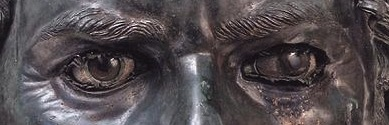
\includegraphics[scale=1]{graphics/seuthesiii.jpg}
	\caption{Detail of 4th century \textsc{bc} Thracian bronze portrait of King Seuthes \textsc{iii}}
	\label{fig:seuthesiii}
\end{figure}

If we suppose the eye to be an animal, perhaps it makes sense to think of the hypothetical creature as possessing the capacity to see. But if we relax that supposition, and consider an eye as it naturally occurs as part of an animal, then it would be wrong to think that an eye possesses the capacity to see. His eyes may have endowed King Seuthes III with the capacity to see, at least when he was alive, but they did not themselves possess this capacity. Similarly amputated eyes, eyes separated from the animal in which they naturally occur as parts, neither possesses the capacity to see nor endow anything else with that capacity. 

There are thus grounds for criticizing a commitment of Empedocles that arises in a passage that, as \citet[211]{Wright:1981zr} observes, Aristotle finds sufficiently interesting to quote three times (in \emph{De Anima} \textsc{iii}.6 430\( ^{a} \)27, \emph{De Caelo} \textsc{iii}.2 300\( ^{b} \)25, and \emph{De Generatione Animalium} \textsc{i}.18 722\( ^{b} \)17):
\begin{verse}
	as many heads without necks sprouted up\\
	and arms wandered naked, bereft of shoulders,\\
	and eyes roamed alone, impoverished of foreheads\\
	(Empedocles, DK \textsc{b}57; \citealt[64 245]{Inwood:2001ve})
\end{verse}
At a certain stage of the cosmic cycle, where Strife still dominates but whose influence is on the wane as Love grows stronger, the parts of animals arise spontaneously and in a disordered state. These combine to give rise to fantastical animals, some with clear mythological precedent:
\begin{verse}
	Many with two faces and two chests grew,\\
	oxlike with men's faces, and again their came up\\
	androids with ox-heads, mixed in one way from men\\
	and in another way in female form, outfitted with shadowy limbs.\\
	(Empedocles, DK \textsc{b}61; \citealt[66 247]{Inwood:2001ve})
\end{verse}
These animals tended not to survive. It is only when animal parts are combined in harmony, due to the increased influence of Aphrodite's Love, do the animals that we presently recognize emerge. Due to the harmony among their parts which fits them to a life in their natural environment, present animals not only survive but have the means of reproduction. Now consider the eyes roaming alone, impoverished of foreheads. Like amputated eyes, they are separated from animals in which they would harmoniously occur as parts. And like amputated eyes, they neither possess the capacity to see nor endow anything else with that capacity. Though eye-like in structure and composition, these are eyes in name only, at least by Aristotle's lights:
\begin{quote}
	What a thing is is always determined by its function: a thing really is itself when it can perform its function; an eye, for instance, when it can see. When a thing cannot do so it is that thing only in name, like a dead eye or one made of stone, just as a wooden saw is no more a saw than one in a picture. (\emph{Meterologica} \textsc{iv}.12 390\( ^{a} \)10--14; Webster in \citealt[86]{Barnes:1984uq})
\end{quote}

The capacity to cut in the manner of axes is a power and potentiality. A thing may possess this power, and so retain the potential to cut in that manner, even when at rest, when it is not actually cutting anything. Similarly, the capacity to see is a power and potentiality. A thing may possess or endow this power, and so retain the potential to see, even when at rest, when it is not actually seeing anything, because of darkness or sleep, say. Aristotle also claims that, in general, matter is potentiality and that form is actuality. There is no inconsistency here as the actual and the potential are said of in many ways. A thing is actually an axe if it possesses what it takes to be an axe, the capacity to cut in the manner of axes, the form and substance of an axe. Moreover the material parts of the thing, the matter of the axe---the wooden shaft, the bronze head---are potentially an axe since they are capable of taking on the form of an axe. When the bronze is suitably fashioned, and honed, and securely fixed to the wooden shaft, the matter, in taking on the form that it does, in so acquiring the capacity to cut in the manner of axes, realizes this potentiality. But what it is to be an actual axe is itself a power and potentiality, the capacity to cut in the manner of axes, a potentiality actualized in so cutting. Similarly, a thing is actually an eye if it possesses what it takes to be an eye, the capacity to see, the form and substance of an eye. Moreover the material parts of the thing, the matter of the eye---the membrane, the interior water---are potentially an eye since they are capable of taking on the form of an eye. When interior water is bound by the membrane and the other parts of the eye are suitably arranged, the matter in taking on the form that it does, in so acquiring the capacity for sight, actualizes this potentiality. What it is to be an actual eye is itself to possess or endow a power and potentiality, the capacity to see, a potentiality actualized in seeing.

The actual and the potential are said of in many ways. In his discussion of these analogies, Aristotle distinguishes two senses of the actual/potential distinction. There is an initial potentiality had by some matter. This potentiality is realized by that matter taking on a form. The taking on of the relevant form is the first actuality. However, in the cases at hand, the relevant form is understood as the possession, or perhaps the endowment of, a capacity. So the first actuality is itself a potentiality. The realization of this potentiality, the exercise of the capacity which is the form of the matter, is the second actuality. These distinctions are schematically represented in table~\ref{tab:potential}

\begin{table}[htbp]
	\centering
		\begin{tabular}{cccc}
			& \emph{An Axe} & \emph{An Eye}\\
			\hline
			\emph{Potenitality} & the matter of an axe & the matter of an eye\\
			\hline
			\emph{First Actuality} & the capacity to cut & the capacity to see\\
			\hline
			\emph{Second Actuality} & cutting & seeing\\
			\hline
		\end{tabular}
	\caption{Two senses of the actual/potential distinction}
	\label{tab:potential}
\end{table}

Eyes endow animals that possess them with the capacity to see. This is a capacity that animals enjoy even when asleep or inattentive. Endowing the perceiver with the capacity for sight is what the organ of sight is for. As \citet{Johansen:1997zr} argues, this further teleological claim motivates a certain explanatory strategy with respect to the anatomical structure of the eye, what he describes as a ``top-down explanation''. Begin with what the organ of sight is for, to endow its possessor with the capacity to see. If the perceiver is endowed with this capacity, then the primary objects of sight, the colors of remote external particulars, potentially appear in the perceiver's experience of them. In order for the colors of remote external particulars to appear in the perceiver's experience of them, the organ of sight must be transparent. Sight is a reactive capacity, the organ of sight must be acted upon for sight to be exercised. And color only ever acts, even mediately, upon what is actually transparent. The eye has the structure and composition that it does to sustain the transparency necessary to endow the perceiver with the capacity for sight. So our initial discussion of transparency (chapter~\ref{cha:transparency}) was necessary not only to understand Aristotle's definition of color (chapter~\ref{cha:color}) but also to understand Aristotle's explanatory strategy with respect to the anatomical structure of the eye. And understanding Aristotle's explanatory strategy, here, will yield insight into the significance of its limitations.



% section the_soul_of_the_eye (end)

\section{Transparency and the Anatomy of the Eye} % (fold)
\label{sec:transparency_and_the_anatomy_of_the_eye}

Why must the organ of sight be transparent?

Sight is a reactive capacity. It is a mode of sensitivity to the colors of remote external particulars. It only acts by reacting to the presence of a particular's color. Since sight is a reactive capacity, it must be acted upon in order for it to be exercised. That its exercise, an episode of seeing, just is being acted upon in this way is a further claim, that Aristotle denies, \emph{De Anima} \textsc{ii}.5. (For a contemporary defence of this denial see \citealt{Travis:2009fk} and \citealt{Kalderon:2012fk}.) Color could not immediately act upon the eye, since contact would blind the perceiver to the particular and its color. Contact precludes sensation, to be palpable is to be imperceptible. Nevertheless, the color of a remote external particular can act upon the eye mediately, by acting upon the intervening medium. Thus was the moral of Aristotle's criticism of Democritus and Empedocles (chapter~\ref{sec:against_the_empedoclean_principle}). The eye is itself affected by the color's effect on light. Since color is the power to alter what is actually transparent, the eye is affected by color's effect on transparent media by itself being transparent, at least in part. They eye is transparent, then, at least in part, so that the colors of remote external particulars may mediately act upon it. Which they must be capable of doing, since sight is a reactive capacity, a mode of sensitivity to the colors of remote external particulars arrayed in the natural environment.

Suppose that is right. Suppose that sight could only be the reactive capacity that it is, a chromatic sensitivity, if the organ of sight were transparent, at least in part. This would constrain its elemental composition. Whereas some elements are receptive to the presence and activity of the fiery substance, such as air and water, other elements, such as earth, exclude the fiery substance or at least retard its activity. Transparency is present only in matter with a certain elemental composition, one that allows for the presence and activity of the fiery substance.

That sight is a reactive capacity, a chromatic sensitivity, not only constrains the elemental composition of the eye, but it also constrains its structure. Transparency is a nature or power common to different substances such as water and air. So the requirement that the internal medium of the eye be transparent does not by itself determine whether an eye must have either elemental composition. Further material considerations determine that the internal medium be water:
\begin{quote}
	True, then, the visual organ proper is composed of water, yet vision appertains to it not because it is water, but because it is transparent---a property common alike to water and to air. But water is more easily confined and more easily condensed than air; it is that the pupil, i.e. the eye proper, consists of water. (\emph{De Sensu} \textsc{ii} 438\( ^{a} \)13--18)
\end{quote}
Air and water are liquids and so lack fixed boundaries. If the organ of sight is thus composed, at least in part, of the transparent, this liquid must somehow be confined to the organ of sight, by a fine membrane (like the membrane with which Aphrodite's Love enshrouds the primeval fire in the eye's interior, Empedocles DK 84). That this is more easily done with water than air favors the conclusion that the eye is composed, at least in part, of water. However, what is presently important is that reflection on the material constraints of sustaining an internal transparent medium not only determines the elemental composition of the internal medium but also significant anatomical structure, the existence of a membrane that confines and condenses the internal water.

That the eye is composed of water, at least in part, receives additional empirical support from gross anatomical observation. Water flows from decomposing eyes (\emph{De Sensu} \textsc{ii} 438\( ^{a} \)17), and this water is remarkably cold and glistening when it flows from the eyes of embryos (\emph{De Sensu} \textsc{ii} 438\( ^{a} \)18). Whereas in sanguineous animals, the eye contains fat and oil to prevent the water from freezing, the eyes of bloodless animals are covered for the the same reason (\emph{De Sensu} \textsc{ii} 438\( ^{a} \)20--3).


Aristotle's anatomy of the eye recapitulates important aspects of the ingestion model, as presented in the answer in the style of Gorgias (\emph{Meno} 76\( ^{a-d} \)):
\begin{quote}
	Now, as vision outwardly is impossible without light, so also it is impossible inwardly. There must, therefore, be some transparent medium within the eye, and, as this is not air, it must be water. The soul or its perceptive part is not situated at the external surface of the eye, but obviously somewhere within: whence the necessity of the interior of the eye being transparent, i.e. capable of admitting light. And that it is so is plain from actual occurrences. It is matter of experience that soldiers wounded in battle by a sword slash on the temple, so inflicted as to sever the passages of the eye, feel a sudden onset of darkness, as if a lamp had gone out; because what is called the pupil, i.e. the transparent, which is a sort of lamp, is then cut off. (\emph{De Sensu} 438b7-438b15)
\end{quote}
This passage is the culmination of a dialectic that began at \emph{De Sensu} 437\( ^{b} \)11. An explanation of vision in terms of the eye's fiery emission, attributed to Empedocles and Plato in the \emph{Timaeus}, is contrasted with the competing explanation of Democritus in terms of the eye's reflection. The passage presents a complex dialectical refinement of the \emph{endoxa}. The explanations of Empedocles and Democritus are, of course, rejected. Importantly, however, Aristotle retains elements of each of their explanations, even if these elements are fundamentally reconceived.

According to Aristotle, Democritus maintains that the eye sees because of its reflective surface, itself due to the smoothness of the eye and the presence of lachrymal fluid (\emph{De Sensu} 438\( ^{a} \)5--12). Democritus is wrong in thinking that this was due to water's capacity for reflection, and consequently wrong in taking the locus of sight to be on the surface of the eye. Nevertheless, Democritus was right to link the eye's capacity to see with the presence of water. However, it is not the reflectivity but the transparency of the eye's water that is required to endow its possessor with the capacity to see. 

% If Democritus was right in thinking that the eye is composed of water, then Empedocles was wrong in thinking that the eye contained fire. This should not obscure for us the way in which Aristotle retains important elements of the Empedoclean theory of vision.

This parallels the way that Empedocles accommodates the dominant medical opinion of his time (discussed in chapter~\ref{sec:empedocles_theory_of_vision}). The presence of lachrymal fluid is both necessary for sight and necessary for the reflective appearance of the eye. This encouraged the opinion that the reflective appearance of the eye explained the eye's receptivity to sight, and hence that the surface of the eye is the locus of sight. However, on the ingestion model, the assimilation of chromatic effluences is a material precondition for their presentation to the organ of sight. On the ingestion model, sight is located within. By conceiving of the receptors on the surface of the eye as water-bound passages to its interior, Empedocles reconciles the ingestion model with the dominant medical opinion of his time. Similarly, Aristotle asserts that ``the soul or its perceptive part is \ldots\ obviously within'' (\emph{De Sensu} \textsc{ii} 438\( ^{b} \)9--10). And like Empedocles, Aristotle retains something of Democritus opinion. But not by finding a role for the surface of the eye in seeing, but by claiming that the eye is partly composed of water. However, as we shall see, the transparent plays a role similar to the role played by ocular passages in Empedocles's theory of vision.

Aristotle rejects the explanation of vision in terms of the eye's fiery emission. While Aristotle attributes this view to Empedocles on the basis of the lantern analogy (DK 84; quoted in full at \emph{De Sensu} \textsc{ii} 437\( ^{b} \)27--438\( ^{a} \)3), he also writes:
\begin{quote}
	Sometimes he accounts for vision thus, but at other times he explains it by emanations from the visible objects. (\emph{De Sensu} \textsc{ii} 438\( ^{a} \)3--4)
\end{quote}
As discussed in chapter~\ref{sec:empedocles_theory_of_vision}, Aristotle thinks that Empedocles is potentially offering distinct explanations of color vision---one in terms of the eye's emission of fiery effluence and the other in terms of the eye's assimilation of chromatic effluences. While Aristotle rejects the explanation of color vision in terms of the eye's fiery emission, he reinterprets Empedocles' lantern analogy on the model of the answer in the style of Gorgias, though with crucial refinements.

While rejecting the explanation of vision in terms of the eye's fiery emission, nowhere does Aristotle directly deny the fundamental claim of Empedoclean a\-nat\-o\-my that the eye is composed of ``fire and its opposite'' (Theophrastus, \emph{De Sensibus}, \textsc{xv}). Perhaps, this is not an omission on Aristotle's part but intentional, for there is another way to understand Empedocles talk of interior fire. If the eye's interior is composed of confined and condensed water in order to sustain its transparency, then the interior water, being transparent, is receptive to the presence and activity of the fiery substance. The external medium must be illuminated if the color of a remote external particular is to be visible in it. Similarly, for that color to be visible, the external light must be extended within. The transparent water of the eye's interior must itself be illuminated. And the internal medium is only illuminated by the presence and activity of the fiery substance. While seeing the white of the sun may not involve the assimilation of fiery effluences as Empedocles maintained, nevertheless, if the white of the sun is visible to the perceiver, this is due, in part, to the presence and activity of the fiery substance in the eye's interior. This is why Aristotle makes the deliberate allusion to Empedocles' lantern analogy (DK 84). Like Empedocles, Aristotle compares the eye to a lantern. But not because the eye emits fire the way a lantern does. But because the interior of the eye must be illuminated, the way the interior of a lamp is illuminated, if the external scene is to be visible. So not only does Aristotle retain the phenomenological insight of Empedocles, that seeing is a mode of assimilation, ``the soul or its perceptive part'' within. But Aristotle also retains the Empedoclean doctrine that the exercise of the capacity for sight involves fire in the eye's interior, understood as the fiery substance illuminating the internal medium. 

Though Aristotle reinterprets Empedocles' lantern analogy on the model of the answer in the style of Gorgias, there are crucial refinements, as he rejects the theory of effluences. 

According to Empedocles, what is assimilated is a material particular, a chromatic effluence, conceived as a fine body, composed of fire or water, with a distinctive magnitude. On Aristotle's reinterpretation of the lantern analogy, what is assimilated is not a material particular, but the state of the external medium, a state sustained by the illuminating presence and activity of the fiery substance. The state of the internal medium need not be the same as the state of the external medium. Internal and external media may differ in their degree of transparency, and so dark eyes may be illuminated to a lesser degree than the surrounding air. Nevertheless, the state of illumination of the interior water is determined by the amount of fiery substance encountered in the external medium and the degree of transparency of the internal medium, the degree to which it is susceptible to the illuminating presence and activity of the fiery substance. 

Despite rejecting the theory of effluences, the transparency of interior water plays, for Aristotle, a function that ocular passages play in Empedocles' theory of vision. Chromatic effluences, because of their distinctive magnitudes, are commensurate with ocular passages. As such, they can travel through such passages and so be palpable to the organ of sight. While a state lacks location, and so cannot travel, the external light is extended within, in the sense in which it can, so that the color of remote external particulars may be present in visual consciousness. It is thanks to the illuminated state of the eye's interior that the perceiver is able to assimilate the chromatic form of distal particulars in the natural environment. As I argued in chapter~\ref{sec:the_answer_in_the_style_of_gorgias}, the assimilation of chromatic effluences by the organ of sight is not, by itself, the sensing of colors. The assimilation of chromatic effluences is at best a material precondition for their sensing. Similarly, admitting light into the interior of the organ of sight is not, by itself, the sensing of colors. Interior illumination is at best a material precondition for their sensing. Sensing is the presentation of the color to the perceptive part of the soul, not by being palpable, but by the assimilation of chromatic form, by the color of remote external particulars shaping visual consciousness. However the doctrine of the assimilation of sensible form is to be understood, interior illumination is a material precondition for sensing, so understood. That the interior illumination takes on a character that depends on derives from the character of the exterior illumination may make the colors of remote external particulars perceptually available, but the perceptually availability of the colors only involves the colors being potentially perceived, not their actual perception.  

% This is another aspect of the ingestion model that is preserved in Aristotle's dialectical refinement of Empedocles' theory.

The present understanding of Aristotle's deployment of the lantern analogy is further confirmed by the empirical evidence that Aristotle marshals at the end of this passage (\emph{De Sensu} 438b12-15). That the eye must be ``capable of admitting light \ldots\ is plain from actual occurrences'', such as the blindness resulting from a wound sustained by a slash on the temple. Such a wound severs passages leading away from the eye and so impairs the eye's capacity to endow its possessor with sight. Though the wounded soldier's eyes are filled with light, since the passages leading within (presumably, to a position at or near the heart) are severed, the colors of remote external particulars are no longer present in his visual consciousness. While they appear through the internal medium, being actually transparent, the colors of distal particulars are cut off from the perceptive part of the soul. The wounded soldier can no longer assimilate the chromatic form of remote material particulars.

We have here another significant part of the eye's anatomy, the passages from the eye leading within. One should not anachronistically assume that Aristotle has in mind the optic nerve. Given that the seat of sensation is at or near the heart, a better hypothesis would be that they are vessels leading to the heart. However, Aristotle's description of these passages underdetermines any such identification \citep[see][]{Lloyd:1978fk}. In fact, Aristotle seems only interested in this anatomical detail insofar as these passages extends the transparent within. In extending the transparent within, the perceptive part of the soul becomes receptive to the direction of influence of the fiery substance. It is the presence and activity of the fiery substance that determines the sensible character of internal and external media. Moreover, the sensible character of transparent media is itself determined by the colors of the particulars that appear through that media. The precise content of the Aristotelian doctrine of the assimilation of sensible form remains, at this point, unclear. What is clear is that, first, it does not involve chromatic forms traveling in the manner of effluences, as \citet[\textsc{i} 1]{Hobbes:1651fk} imagined, and that second, the passages extending the eye's transparency within are necessary for the assimilation of chromatic form. 

Not only does Aristotle's empirical example provide us with another significant part of the eye's anatomy, but it also further illustrates what \citet{Johansen:1997zr} describes as Aristotle's ``top-down explanation''. Sight is the soul of the eye, or it would be if it were an animal. Endowing its possessor with the capacity for sight is what the organ of sight is for. Consequently the organ of sight is understood to have the structure and composition required to endow this capacity. Evidently, passages extending the transparent within are necessary for the capacity for sight, since when they are severed, the victims of such wounds are blinded. We have an explanation from what the organ of sight is for---to endow the perceiver with the capacity for sight---to anatomically significant structure---passages leading away from the eye.

So far we have distinguished the condensed and confined water in the eye's interior, the membrane that confines it, the pupil, and passages leading away from the eye to some point in the interior, perhaps, at or near the heart. In addition, Aristotle distinguishes the dark of the eye from the light (\emph{De Sensu} \textsc{ii} 437\( ^{b} \)1), understood as the iris and the white of the eye that surrounds the iris (\citealt[see][218, 231 n13]{Lloyd:1978fk}). In sanguineous animals, the white is fat and oily to prevent the transparent water of the eye from freezing (\emph{De Sensu} \textsc{ii} 438\( ^{a} \)20--3). The contrast must be with the dark of the eye, as opposed to the black, since Aristotle recognizes different colored irises: ``In some it is black, in some distinctly blue, in some greyish-blue, in some greenish'' (\emph{Historia Animalium} \textsc{i}.10 492\( ^{a} \)2--3). Blue, grayish-blue, and greenish may be dark, at least when compared with the white of the eye, but they are not black. Further evidence, if any were needed, that \emph{melaton} and its cognates should be understood as dark as opposed to black in the Aristotelian color scheme.

The Aristotelian anatomy of the eye is crude, even by ancient standards. Lloyd summarizes its limitations:
\begin{quote}
	Yet no attempt is made to describe the structure of the eye as a whole, although this is, of course, complex. The three main parts Aristotle identifies quite incidentally in the course of this chapter, pupil, iris, white, relate primarily to the superficial appearance of the eye. Apart from the one reference to the membrane of the eye and the one reference to certain \emph{poroi}, already mentioned, his remarks on the internal structure of the eye are confined to the point that the pupil, \emph{kore}, consists of water. We may take it that this refers to the vitreous humour that occupies most of the bulb of the eye and which, in certain lesions, might produce a watery discharge. But there is no mention of the membrane enveloping the vitreous humour (retina, choroid, sclera), nor of the lens, nor of the anterior chamber between the cornea and the lens. There is, in fact, no mention of most of the parts that seem difficult to identify straightforwardly as water, and no systematic description of the internal structure of the eye as such at all. \citep[220--221]{Lloyd:1978fk}
\end{quote}
While the Aristotelian anatomy of the eye can be further refined and extended (and was by the commentators---Philoponus recognized the anterior chamber between the cor\-nea and the lens), important limitations will inevitably remain. The significance of these limitations should be judged in relation to the specific explanatory concerns Aristotle and the Peripatetic tradition were addressing in articulating the eye's anatomy. \citet{Lloyd:1978fk} takes Aristotle to be primarily addressing the problem of how to assign the four elements to the five senses. This is indeed a task of \emph{De Sensu}. But as I have argued, Aristotle has more specific explanatory concerns. The eye must have such a nature so as it may be mediately acted upon by color in order to endow its possessor with the reactive capacity for sight. Taken by itself, this claim is the expression of a reasonable explanatory strategy. If Aristotle's anatomy of the eye strikes us as superficial or schematic, this is not due to this explanatory strategy alone, nor is it due to an abstract taxonomic concern with assigning elements to senses. Rather, two further claims are responsible for the limitations of Aristotelian anatomy: (1) that the eye can only be mediately acted upon if it is actually transparent, and (2) that the eye is only acted upon by altering the character of its interior illumination. Whereas (1) specifies a condition on the patient of change, (2) specifies the nature of the change. It is these further commitments that lead him to discern only those parts of the eye that might plausibly be said to play a role in sustaining the transparency of the internal medium.


% section transparency_and_the_anatomy_of_the_eye (end)

\section{Interior Illumination} % (fold)
\label{sec:interior_illumination}

The eye in seeing is like a lantern, not because it emits fire from its interior, but because in seeing the interior of the eye is illuminated. The confined and condensed water in the interior of the eye is transparent for the sake of receiving such illumination. It is only be being transparent that colors can mediately act upon the eye by acting upon the intervening medium. And since sight is a reactive capacity, a mode of chromatic sensitivity, the organ of sight must be acted upon if the capacity for sight is to be exercised in seeing the presented color.

What is the effect that the color produces in mediately acting upon the eye?

Since color acts upon the eye by acting upon the external me\-di\-um, the effect on the internal medium should be of the same kind as the effect that color has on the external medium. Aristotle explicitly speaks of admitting light. Colors affect the character of the illuminated medium, so in admitting light, the transparent medium within the eye not only must be actually transparent, due to the illuminating presence and activity of the fiery substance, but it must also come to have a character that at least corresponds to the character of the external illuminated medium. The correspondence need not be identity. As we observed, internal and external media may differ in their degree of transparency, and so dark eyes may be illuminated to a lesser degree than the surrounding air. The light admitted by dark eyes, their interior illumination, will not be as bright as the exterior illumination. Nevertheless, the existence and character of the interior illumination depends upon and derives from the existence and character of the external illumination that immediately acts upon it.

This places an important metaphysical constraint on the character of the interior illumination. Whatever effect color has on the external medium, such as the surrounding air, the external medium has a corresponding effect on the internal medium. In chapter~\ref{sec:the_definition_of_color}, we reviewed some candidate effects. Given the metaphysical constraint, the candidate effects on the internal medium, the illuminated water in the eye's interior, correspond to these.

In chapter~\ref{sec:the_definition_of_color}, I argued that color could not color external media since doing so would be inconsistent with the way that colors are perceptually available within them---either by being inconsistent with the medium being actually transparent or by being inconsistent with the directionality of the visible. The agent of a change must actually be the way that the patient potentially is. Insofar as the external medium acts upon the internal medium---light is admitted---the external medium is an agent of change, the internal medium the patient. Since the external medium could not be colored, in admitting light, the internal medium, the transparent water within the eye's interior, could not in turn be colored. This result is one of the advantages of the present mode of exposition, focused fundamentally on the nature of the transparent, that begins with color's effect on external transparent media before considering color's mediate effect on internal transparent media.

As before, three candidate effects remain:
\begin{enumerate}[(1)]
	\item The rendering visible of the transparent---making the transparent internal me\-di\-um perceptually available
	\item The rendering visible of colored particulars arrayed in the transparent external me\-di\-um\----making the colored particulars perceptually available
	\item Affecting the fiery substance by affecting the amount of it in the internal me\-di\-um, the water within the eye, or, if this does not come to the same thing, promoting or retarding its activity to some degree, or otherwise affecting its direction of influence
\end{enumerate}
(1) follows from the \emph{De Anima} (\textsc{ii}.7 418\( ^{b} \)4--6) definition of the transparent. It might seem odd to claim that the transparent water in the eye's interior is perceptually available to us, even when illuminated. However, recall, by Aristotle's definition of transparency, the transparent appears to us by the colors of remote external particulars appearing through it. Since when we see the colors of remote external particulars, we see them through the transparent medium in the eye's illuminated interior, we see that medium as well. Of course, ordinarily we do not attend to the transparency of the eye's interior water until it is disrupted, when we see floaters, say. But, in seeing the colors, the internal medium must itself be perceptually available, at least in the manner of transparent things enshrined in the \emph{De Anima} definition of transparency. (2) is not only a consequence of the \emph{De Anima} definition, but is a commitment of Aristotle's description of the wounded soldier. That the colored particulars arrayed within the transparent external medium are perceptually available within the water in the eye's interior is demonstrated by severing the illuminated interior from the perceptive part of the soul, located at or near heart. When the transparency in the eye's interior is no longer extended within, the passages leading from the eye having been severed by a sword's blow, the colors of remote external particulars are no longer perceptually available. The soldier has been blinded by his wound. (3) not only draws upon materials available in both \emph{De Anima} and \emph{De Sensu}, but coheres well with the \emph{De Sensu} project of explaining what each of the sense object must be to produce the sensation in full actuality. (1) and (2) are psychological effects in that perceptual availability is or involves potential perception. (3) is not psychological, even in this extended sense, but is, rather, a material change. These psychological and material changes need not be inconsistent. They may be part of formal and material explanations of the same phenomena. 

Given the proportion of the transparent that exists in all bodies, colored particulars have the power to affect the amount, activity, and direction of influence of the fiery substance in illuminated media. In so affecting the fiery substance, the particular, or at least its color, is perceptually available. In acquiring the power to affect light in a certain way, the colored particular also acquires the power to mediately affect the eye, the organ of sensation sensitive to such alterations in illuminated media. When the transparent water in the eye's interior is suitably aligned to the direction of influence of the fiery substance illuminating the external medium, interior water is immediately illuminated, 

% If color vision is a mode of sensitivity to the chromatic form of remote external particulars, the organ of sight must be acted upon

% section interior_illumination (end)

% chapter the_eye (end)

%!TEX root = /Users/markelikalderon/Documents/Git/formwithoutmatter/formwithoutmatter.tex
\section{Two Transitions to Actuality} % (fold)
\label{sec:two_kinds_of_potentiality}

% section two_kinds_of_potentiality (end)

\section{Form Without Matter} % (fold)
\label{sec:form_without_matter}

% section form_without_matter (end)

% Nocite
\nocite{Inwood:2001ve}

% Bibligography
\bibliographystyle{plainnat} 
\bibliography{Philosophy} 

\end{document}
